% La parte central del trabajo refiere a lo que es producción propia o aporte del
% proyecto de grado, incluyendo las decisiones tomadas. Por ejemplo, puede incluir
% los requerimientos, el análisis y el diseño de la solución. Si el proyecto tiene una
% implementación, debe describirse en términos de decisiones tomadas en ese sentido.
% Los detalles de programación se dejan para los anexos.

% Se pueden incluir figuras en el documento, las mismas deben estar referenciadas en el texto. Por ejemplo, la Figura~\ref{fig:logos} muestra los logos de Facultad de Ingeniería y de la Universidad de la República.

% \begin{figure}[h!]
%     \centering
%     
\includegraphics[width=\textwidth]{figs/logo-udelar-fing.png}
%     \caption{Logos de FIng y UdelaR}
%     \label{fig:logos}
% \end{figure}

\graphicspath{{chapters/3_diseño/figures/}}

% parte central
\chapter{Voxel cone tracing}\label{chap:design}

En este capítulo se detalla el diseño de \textit{voxel cone tracing} \cite{voxel-cone-tracing}, un algoritmo de iluminación global en tiempo real, que utiliza conceptos presentes en el trazado de rayos (\ref{sec:ray-tracing}), trazado de conos (\ref{sec:historical-cone-tracing}) y \textit{photon mapping} (\ref{sec:photon-mapping}), 
pero reduciendo los costos asociados a estos algoritmos clásicos usando una representación de la escena con vóxeles (\ref{sec:vóxeles}), almacenada en un \textit{octree} disperso (\ref{sec:octree}), para aproximar los conos.

Otra forma de reducir costos y aumentar la velocidad del algoritmo es utilizando el ducto de rasterización \ref{sec:graphics-pipeline} y renderizado diferido \ref{sec:deferred-rendering}.
Los cálculos de luz se realizan en el \textit{fragment shader} del ducto de raster, sobre los \textit{geometry buffers} para reducir la cantidad de fragmentos o hilos de la gpu sobre los que se corren calculos pesados, sin perder calidad de imagen.
Lo anteriormente explicado difiere del trazado de rayos clásico, que renderiza toda la escena puramente mediante intersecciones entre rayos y geometría.

% TODO: Este párrafo es nuevo, así que hay que darle una pasada
La principal aproximación que realiza este algoritmo es trabajar sobre una representación voxelizada pre-filtrada de la escena.
Dadas las coordenadas de un punto de la escena, se recorre el árbol para hallar el vóxel que representa la región del espacio que incluye ese punto.
Este vóxel contiene toda la información necesaria sobre oclusión, color e irradiancia debido a que la estructura es previamente filtrada.
En el filtrado, la información en las hojas del árbol es promediada hacia niveles mayores hasta que cada nivel del árbol contiene información que aproxima las capas inferiores.
La información de un vóxel en cada nivel resume la información de los vóxeles de los nodos hijos que comparten el mismo espacio en la escena.
Se vió en la sección sobre trazado de conos (\ref{sec:ray-tracing}), que en su planteo original, se hallaban las intersecciones del cono con los objetos de la escena de manera analítica, lo que es costoso.
Aquí, en lugar de hallar la intersección analiticamente, se aproxima el cono utilizando la estructura jerárquica de vóxeles lo cual permite acumular la información a lo largo del cono mas eficientemente, pero con cierta perdida de detalle.

% TODO: Estaría bueno poner diagramas de cada etapa:
% - Voxelización: no se qué hacer
% - Construcción y filtrado
% - Inyección de fotones: puedo poner un dibujo de rayos saliendo de la fuente de luz
% - Trazado de conos: poner un cono agarrando varios vóxeles

El algoritmo se puede dividir en 4 grandes etapas:

\begin{enumerate}
    \item Voxelización de la escena
    \item Construcción y filtrado del \textit{octree} disperso
    \item Inyección de fotones
    \item Trazado de conos
\end{enumerate}

La voxelización, la inyección de fotones y el trazado de conos usan el ducto de rasterización, mientras que la construcción del árbol y el filtrado usan el ducto de cómputo de propósito general.
En el resto del capítulo se explicará con mayor grado de detalle cada una de estas etapas.

\section{Voxelización}\label{sec:voxelization}

La escena se divide en una grilla de vóxeles.
La cantidad de vóxeles es configurable, siendo usualmente $512$ o $1024$ por dimensión, lo cual lleva a un total de $512^3$ o $1024^3$ vóxeles respectivamente.

Para voxelizar la escena, se realiza el procedimiento detallado en ``OpenGL Insights, capítulo 22'' \cite{opengl-insights}, un aporte escrito por Crassin luego de haber publicado el artículo de \textit{voxel cone tracing}, aprovechando mejoras en las herramientas disponibles en el momento.
Ese mismo proceso será explicado a continuación, para más información, consultar la referencia.

Usando el ducto de rasterización de OpenGL, se procesan todos los triángulos de la geometría de la escena utilizando como resolución para el rasterizado la resolución de la grilla de vóxeles.
Esto genera una lista de \textbf{vóxeles}, donde cada voxel es una posición dentro de la grilla y un color, el cual es el color de un triangulo que interseca con el espacio representado por el voxel.
Cada uno de estos vóxeles será usado para construir el árbol y terminará almacenado en la estructura. Dado lo anteriormente descrito, el mismo voxel, identificado por su posicion en la grilla, puede estar presente en al lista multiples veces con colores diferentes si mas de un triangulo interseca con el voxel. 

La voxelización de un triángulo $B$ a un vóxel $V$ puede hacerse si:

\begin{enumerate}
    \item El plano de $B$ interseca $V$.
    \item La proyección 2D del triángulo $B$ por la dimensión dominante de su normal (la que provee la mayor área proyectada) interseca la proyección 2D de $V$.
\end{enumerate}

Basado en esta observación, se sigue la serie de pasos que se muestra en la figura \ref{fig:voxelization_pipeline}.

\begin{figure}[h!]
    \centering
    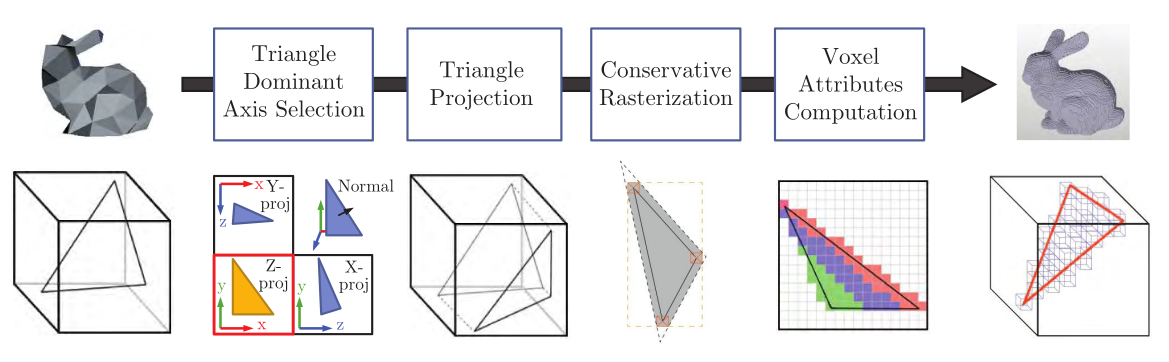
\includegraphics[width=\textwidth]{voxelization_pipeline.png}
    \caption{Ducto de voxelización. Fuente: \cite{opengl-insights}}
    \label{fig:voxelization_pipeline}
\end{figure}

Primero, cada triángulo de la geometría se proyecta ortográficamente en la dimensión dominante de su normal.
La dimensión dominante se elige dinámicamente por triángulo en el \textit{geometry shader}, donde la información de los tres vértices de cada triángulo está disponible,
maximizando el area del triangulo proyectado.

Cada triángulo proyectado se rasteriza para conseguir fragmentos correspondientes a la resolución 2D de la grilla de vóxeles.
Se fija el tamaño del \textit{viewport} a coincidir con la cantidad de vóxeles, por ejemplo un \textit{viewport} de tamaño $512\times512$ para una grilla de $512^3$ vóxeles.
% Mientras se hace esto, se mantienen las operaciones del framebuffer desactivadas, como el depth testing. % TODO: Habría que explicar por qué, no entendí del capítulo de OpenGL Insights. No se por que se desactiva el depth testing, si igual lo que se genera en el frame buffer no se usa, suena como algo de bajo nivel

Durante la rasterización, cada triángulo genera un conjunto de fragmentos 2D. Estos fragmentos corresponderian n a 1 con los vóxeles de la grilla si esta fuese 2D, ya que varios triangulos pueden intersecar con el mismo voxel.
Sin embargo al ser una grilla 3D es necesario calcular la intersección del plano del triangulo con los voxles para encontrar los valores de profundidad en la grilla.
Debido a la elección de la dimensión dominante de la normal para la proyección, solo pueden intersecar con 3 vóxeles en profundidad, por lo que cada fragmento genera de 1 a 3 vóxeles con mismos valores de $x$ e $y$ pero diferentes valores de $z$. % TODO: Por qué? No se explicarlo sin algun dibujo :sweat-smile: Yo tampoco, asi que voy a agregar dibujitos o dejarlo para que nos pregunten porque creo que es de lo que mas me cuesta explicar
Entonces, por cada fragmento 2D, los vóxeles que intersecaron con el triángulo se calculan en el \textit{fragment shader}, basándose en la posición, la profundidad y las derivadas en espacio de pantalla. % TODO: Hacemos lo de las derivadas? Si!

Luego de realizada la voxelización, se obtiene la lista de vóxeles necesaria para crear el árbol, con su posicion y color.
Cada uno tiene una coordenada que lo identifica dentro de la grilla 3D de la escena, así como color y posición en el espacio de la escena.

\subsection{Rasterización conservativa}

El método descrito anteriormente a veces no crea vóxeles para elementos muy finos, como un asta de bandera ya que en el rasterizado solo se prueba el centro del píxel contra los triángulos para generar fragmentos. % TODO: Revisar en el código
Se necesita una manera de generar fragmentos para cada píxel tocado por un triángulo, no necesariamente en el centro.
Un algoritmo así se detalla en \cite{conservative-rasterization}.

La idea es generar, por cada triángulo, un polígono acotante ligeramente más grande, para asegurarse que cualquier triángulo proyectado que interseca con cualquier punto del píxel también interseque con su centro.
Se logra trasladando las aristas del triángulo hacia afuera, la mitad de la diagonal de un píxel, y extendiendolas para generar un triangulo semejante.
A su vez se generan fragmentos nuevos que resultan de sobreestimar la cobertura de este triángulo, dado que este nuevo triangulo puede intersecar con el centro de píxeles que antes no intersecaban en ningun punto.
Para evitar estos fragmentos tambien se genera una caja acotante alineada con los ejes, y se descartan fragmentos por fuera de la misma.
Este proceso se muestra en la figura \ref{fig:conservative_rasterization}.

\begin{figure}[h!]
    \centering
    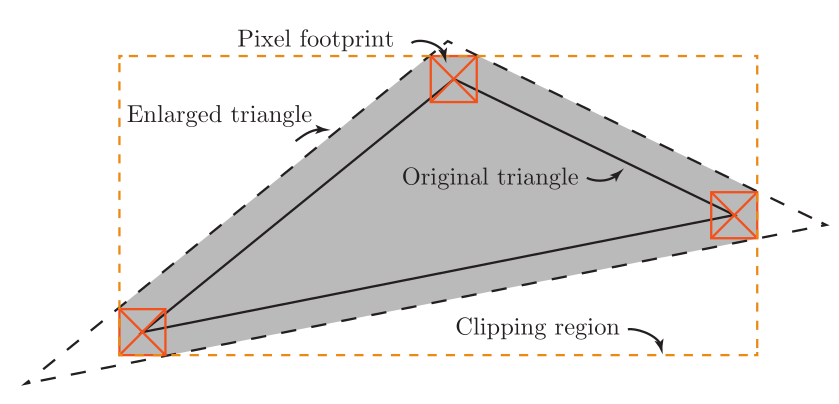
\includegraphics[width=\textwidth]{conservative_rasterization.png}
    \caption{Rasterización conservativa. Fuente: \cite{opengl-insights}}
    \label{fig:conservative_rasterization}
\end{figure}

\section{\textit{Octree} disperso}

Para almacenar los vóxeles generados, se usa un \textit{octree} disperso, como los vistos en la sección \ref{sec:octree}.
Un octree denso subdivide la escena en 8 cubos y cada cubo se subdivide en 8, y asi sucesivamente. Esta estructura puede escalar rápidamente, generando problemas importante de volumen y velocidad de acceso necesarios de memoria.
Para alivianar este problema se crearon los octree dispersos, donde los nodos no se subdividen si no poseen geometría dentro.

Cada elemento del árbol es un \textbf{nodo}.
Un nodo del árbol representa una sección de la escena.
Cada nivel tiene una cierta cantidad de nodos.
Si el árbol fuera denso, cada nivel $n$ tendría $8^n$ nodos.
El nivel $0$ tendría $1$ nodo, el nivel $1$ tendría $8$, el $2$ $64$ y así sucesivamente. % Esto se desprende de lo anterior, pero me parece una simplificacion posiblemente util
El último nivel del árbol es el que llega a la resolución deseada de $512$ o $1024$ vóxeles.
Valores más altos de resolución crean más niveles del \textit{octree} y hacen que se asemeje cada vez más la aproximación de vóxeles a la geometría real.

% TODO: Podría agregar fotos de la visualización del octree a distintas resoluciones

Dado que la estructura tiene como máximo $512$ o $1024$ vóxeles de resolución, sin importar la geometría de la escena, los cálculos sobre ella son independientes de la complejidad de la geometría.

\subsection{Nodos y bricks}\label{sec:nodes_and_bricks}

Los nodos del árbol no almacenan los vóxeles mencionados en \ref{sec:voxelization}.
Cada nodo almacena únicamente un puntero a sus, como máximo $8$, hijos.

Cada nodo tiene asociado un \textbf{brick}, otra estructura que también representa una región del espacio.
Cada brick está dividido en 27 vóxeles, distribuidos en una estructura de $3\times3\times3$ vóxeles.
Son estos vóxeles los que almacenan los valores de la escena.
En la figura \ref{fig:node_and_brick} se puede observar un nodo con su brick asociado de la manera en la que se disponen en el espacio.
Los bricks ocupan más espacio que sus nodos, ya que los vóxeles se centran en los vértices del nodo.
Lo cual es necesario para que los bricks puedan obtener valores de sus vecinos, lo que garantiza que la interpolación dentro de un solo brick toma en cuenta los valores de sus vecinos resultando en una frontera compartida entre vecinos, como se puede ver en la figura \ref{fig:brick_border_overlap}.
La frontera entre dos nodos adyacentes del mismo nivel son los 9 vóxeles de la cara compartida entre los nodos, los cuales estan presentes en los bricks de ambos nodos, lo cual es necesario para que la interpolación a la hora de generar la imagen final funcione.
Un \textit{shader} llamado \textit{border\_transfer}, es el que se encarga de lograr la coherencia en la frontera entre dos \textit{bricks}.
Se explicará en la Sección \ref{sec:border_transfer}.

\begin{figure}[h!]
    \centering
    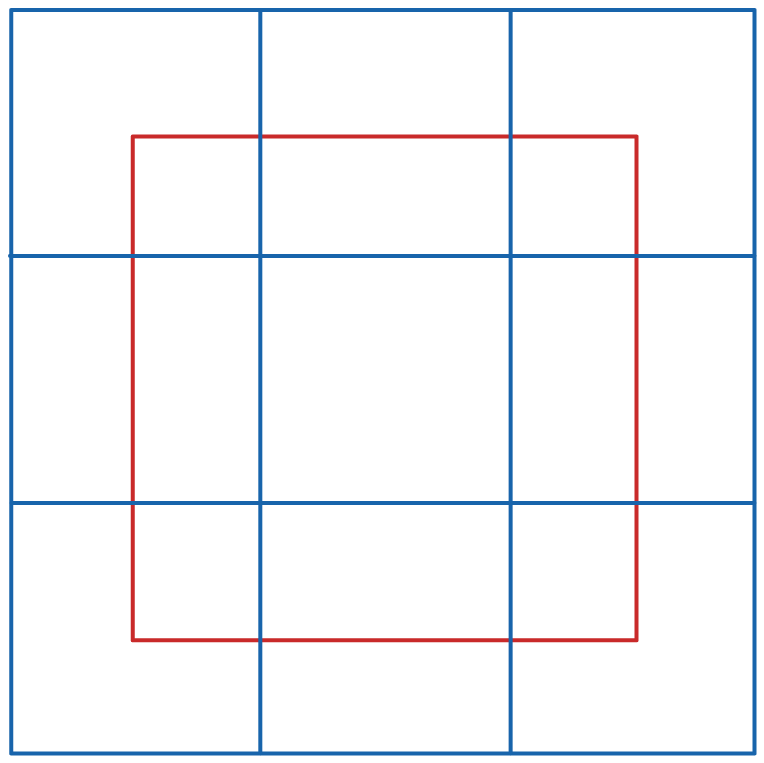
\includegraphics[width=.3\textwidth]{node-and-brick.png}
    \caption{Nodo (en rojo) con su brick asociado (azul)}
    \label{fig:node_and_brick}
\end{figure}

\begin{figure}[h!]
    \centering
    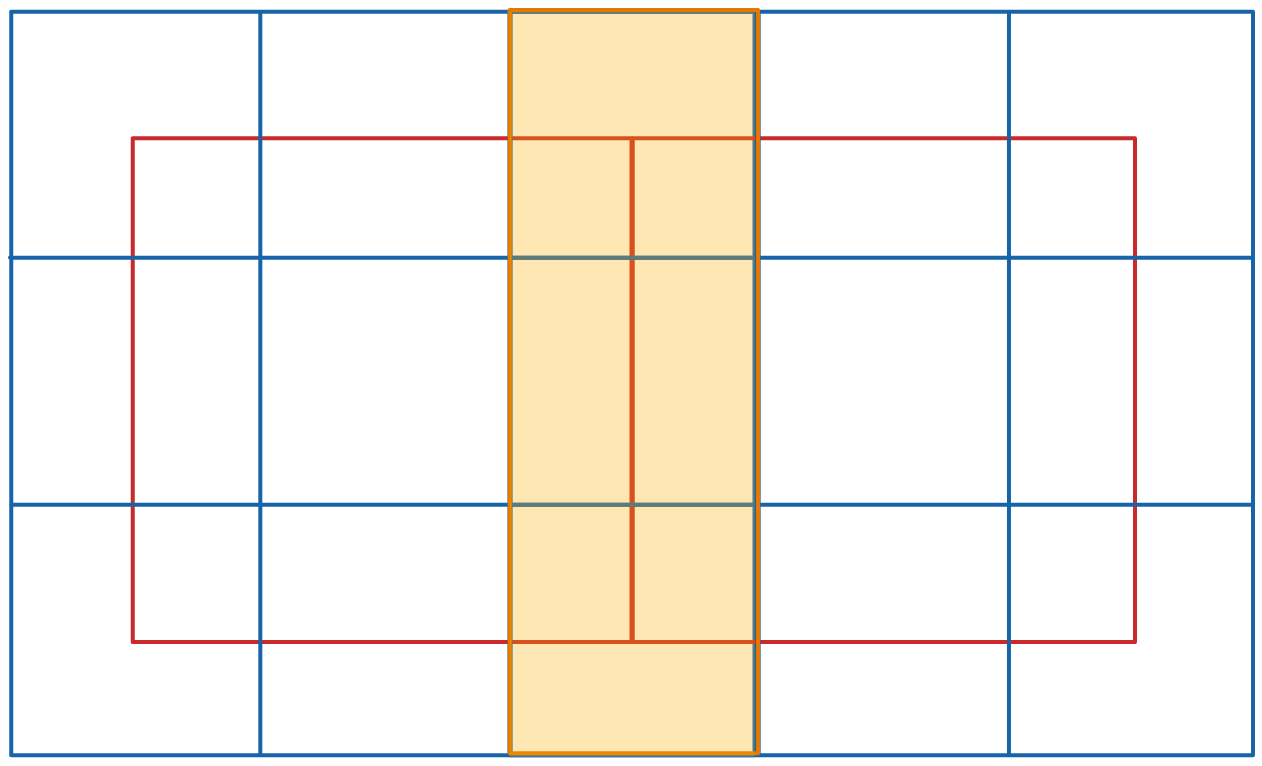
\includegraphics[width=.5\textwidth]{brick-border-overlap.png}
    \caption{Solapamiento entre vóxeles de bricks de nodos vecinos}
    \label{fig:brick_border_overlap}
\end{figure}

\subsection{Construcción}\label{design:svo_construction}

Para generar el octree disperso se usa la lista de vóxeles generada durante la voxelización.
Se empieza con un árbol con un solo nivel, con un solo nodo que ocupa toda la escena.
Se ejecuta el algoritmo a continuación sobre cada nivel para generar el siguiente hasta completarlo.

% TODO: Dibujos para explicar flag y allocate

Dado un nivel $i$ del árbol, dos programas principales son ejecutados en secuencia para generar el nivel $i + 1$: \textit{flag\_nodes} y \textit{allocate\_nodes}.

Se corre un hilo de \textit{flag\_nodes} por cada vóxel de la lista de vóxeles.
Dado un vóxel, se recorre el árbol construido hasta el momento, hasta que se llega a una sección del nodo no subdividida y se marca para ser subdividida.

Luego, se ejecuta \textit{allocate\_nodes}, que busca en el nivel $i$ las secciones marcadas para subdividir.
Al encontrar una sección de un nodo marcada, crea un nuevo nodo en la estructura y cambia la marca por un puntero a ese nuevo nodo.

Siempre y cuando haya geometria en la región de la escena representada por un nodo, la misma será subdividido nivel tras nivel hasta el maximo determinado por la resolución de la grilla de vóxeles.

Una vez alcanzado el último nivel, se escriben los atributos de los vóxeles en los bricks de las hojas del árbol, promediando cuando más de uno tiene la misma posición en la grilla de vóxeles.
Mientras más triángulos tenga la escena original y menos resolución tiene la grilla de vóxeles, mas ocurre lo anteriormente mencionado.
Las hojas no tienen hijos.

% Esto creo que deberia ir en implementacion
En \ref{sec:nodes_and_bricks}, se vió como los bricks ocupan una región más amplia del espacio que su nodo correspondiente.
% TODO: Habría que explicar que los vóxeles son un octavo de nodo del último nivel. Para que esto tenga sentido.
Para consolidar esto con el tamaño de los vóxeles, estos se almacenan únicamente en las esquinas de los bricks. % TODO: Esto esta muy mal explicado
Se almacenan en la esquina más cercana a la posición del vóxel.
Luego, se aplica un programa \textit{spread\_leaves}, para esparcir los valores de las esquinas a lo largo de todo el brick.
Su funcionamiento se muestra en 2D en la figura \ref{fig:spread-leaves}:
\begin{itemize}
    \item El vóxel central almacena el promedio de todas las 8 esquinas
    \item El vóxel del medio de cada cara almacena el promedio de las 4 esquinas de su cara
    \item El vóxel del medio de cada arista almacena el promedio de las 2 esquinas de esa arista
\end{itemize}
Como resultado, se esparcen los valores de las esquinas a todo el brick.
Lo anteriormente descrito es el algoritmo que expande los vóxeles generados poder llenar los bricks $3\times3\times3$.
A partir de aquí, el termino ``vóxel'' refiere a una de las $27$ subdivisiones de un brick, dado que ya se procesó la lista generada durante la voxelización.

\begin{figure}
    \begin{subfigure}{.5\textwidth}
        \centering
        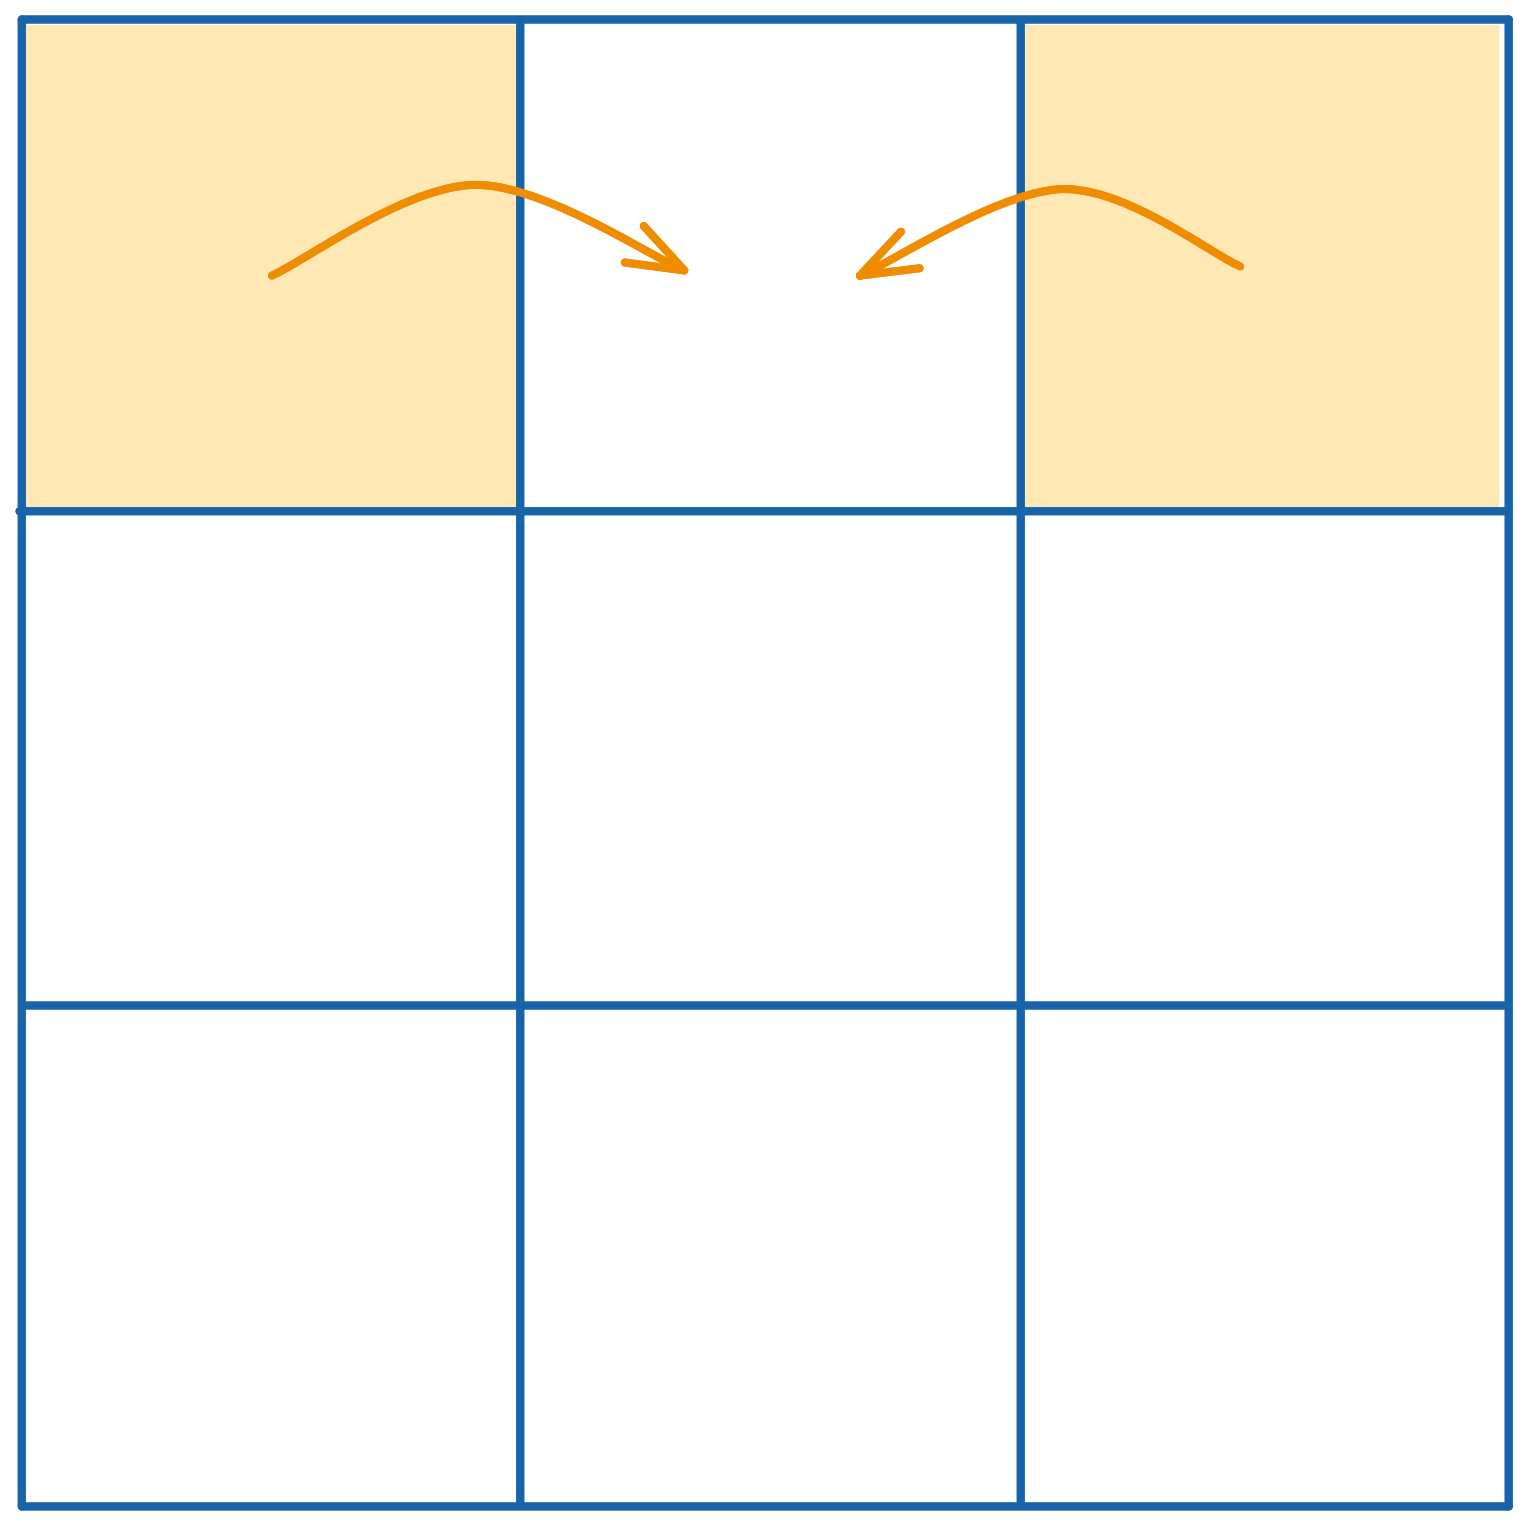
\includegraphics[width=.75\textwidth]{spread-leaves-edge.png}
        \caption{En una arista}
    \end{subfigure}
    \begin{subfigure}{.5\textwidth}
        \centering
        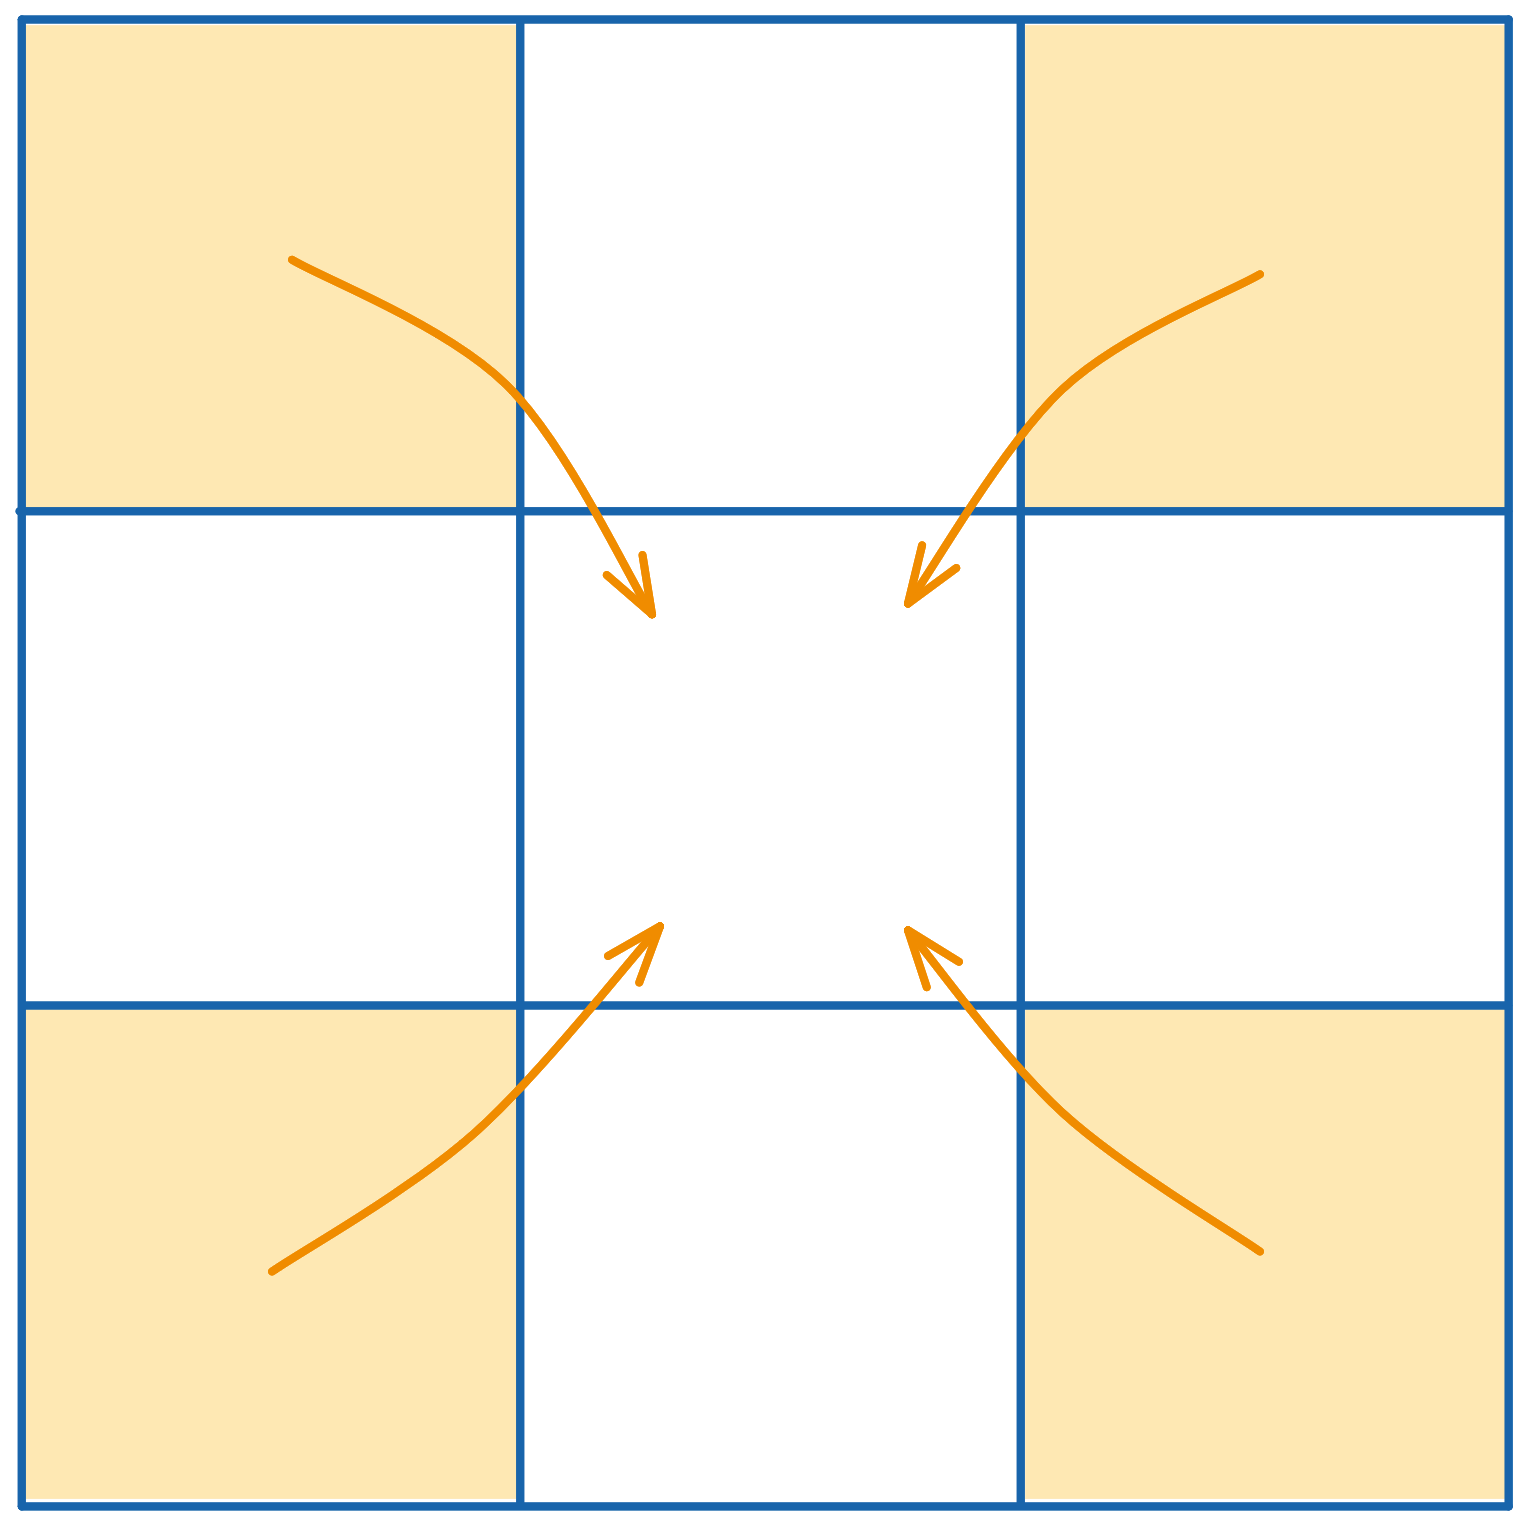
\includegraphics[width=.75\textwidth]{spread-leaves-center.png}
        \caption{En el centro}
    \end{subfigure}
    \caption{Funcionamiento de \textit{spread\_leaves} en 2D. Las flechas indican aporte al promedio}
    \label{fig:spread-leaves}
\end{figure}

\subsection{Border transfer}\label{sec:border_transfer}

Como se mostro en la figura \ref{fig:brick_border_overlap}, las fronteras entre bricks son compartidas, correspondiendo al mismo espacio en la escena.
Por lo tanto, los valores almacenados en esos vóxeles deben ser los mismos garantizando una correcta interpolación a la hora de generar la imagen final.
Sin embargo, luego de aplicar \textit{spread\_leaves}, cada frontera tiene valores distintas en cada par bricks vecinos.
Para igualarlos, se promedian los valores de la frontera con la del brick vecino, asegurandose que el nivel sea coherente.
El shader \textit{border\_transfer} se encarga de promediar los valores en la frontera de cada brick con la de sus vecinos, en X, Y y Z.
De esta manera, aún cuando un vóxel puede estar en varios bricks, en $8$ como máximo, su valor va a ser siempre el mismo en cada uno de ellos. % Creo que tiene razon Eduardo, pero no hay ganas de cambiarlo

% TODO: Dibujos para explicar border transfer

\subsection{Nodos frontera}

Al usar un octree disperso, no existen nodos donde no hay geometría.
\textit{Border transfer} asume que todo nodo tiene un vecino en su mismo nivel en el árbol, lo cual no siempre es verdad.
Por ejemplo en el límite entre la geometría y el espacio vacío existen nodos sin vecino, ya que al ser un árbol disperso no hay nodos donde hay exclusivamente espacio vacio.
Los nodos sin vecino causan un problema, dado que no se puede promediar el valor de sus vóxeles con el vecino, lo que causa problemas de interpolación.
Para que la interpolación continue y logre difuminar el sombreado, es necesaria una capa de nodos extra, los que llamaremos \textbf{nodos frontera}, que representa el espacio vacío adyacente a la geometría.

Los nodos frontera se añaden en cada nivel del árbol a la hora de construírlo.
Sus bricks no contienen valores, existen solo para interpolar los valores con 0 y así difuminar los bordes de la geometría para mejorar la interpolación.
De esta forma los vóxeles compartidos entre espacio vacio y geometría tienen un promedio de ambas, similar al resto de los vóxeles compartidos entre nodos.
El mismo problema no se genera entre estos nodos frontera y el espacio vacio, dado que los vóxeles compartidos con el espacio vacio van a tener como valor la opacidad nula, por lo que se tiene una estructura consistente.

% TODO: Dibujos para explicar nodos frontera

\subsection{Filtrado}\label{design:filtering}

Una vez que todos los atributos se encuentran en las hojas del octree, los mismos seran filtrados a posiciones superiores.
Filtrarlos implica promediarlos de tal manera que para un nodo interior (no hoja) $A$, su brick tenga un promedio de la información contenida en los bricks de todos sus hijos.
El proceso se realiza en $n - 1$ pasos, siendo $n$ el nivel máximo del octree.
En cada paso, se calcula el valor de cada vóxel del brick del padre, usando los bricks de los hijos.

Consideremos un nodo en el penúltimo nivel, con su brick asociado y sus hijos, como muestra la figura \ref{fig:node_with_children}.
En la figuran se muestran solo $4$ hijos porque se usa como ejemplo un cuadtree, la versión 2D del octree, ya que es mas facil de visualizar.
Cada hijo tiene a su vez su propio brick asociado como se muestra en la figura \ref{fig:all_child_bricks}.

\begin{figure}[h!]
    \centering
    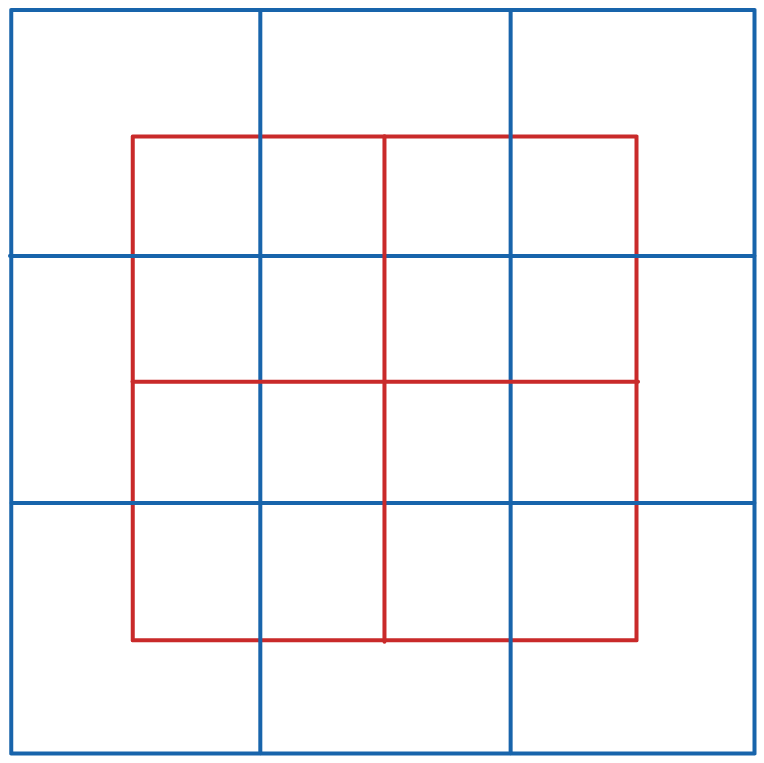
\includegraphics[width=.3\textwidth]{node-with-children.png}
    \caption{Nodo con su brick asociado y sus hijos}
    \label{fig:node_with_children}
\end{figure}

\begin{figure}[h!]
    \begin{center}
        \begin{subfigure}{.24\textwidth}
            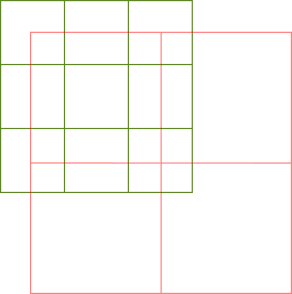
\includegraphics[width=\textwidth]{first-child-brick.png}
        \end{subfigure}
        \begin{subfigure}{.24\textwidth}
            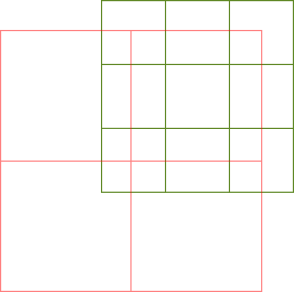
\includegraphics[width=\textwidth]{second-child-brick.png}
        \end{subfigure}
        \begin{subfigure}{.24\textwidth}
            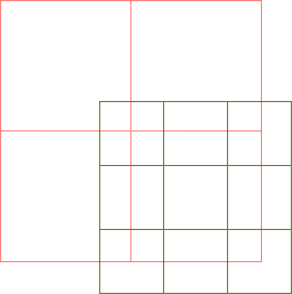
\includegraphics[width=\textwidth]{third-child-brick.png}
        \end{subfigure}
        \begin{subfigure}{.24\textwidth}
            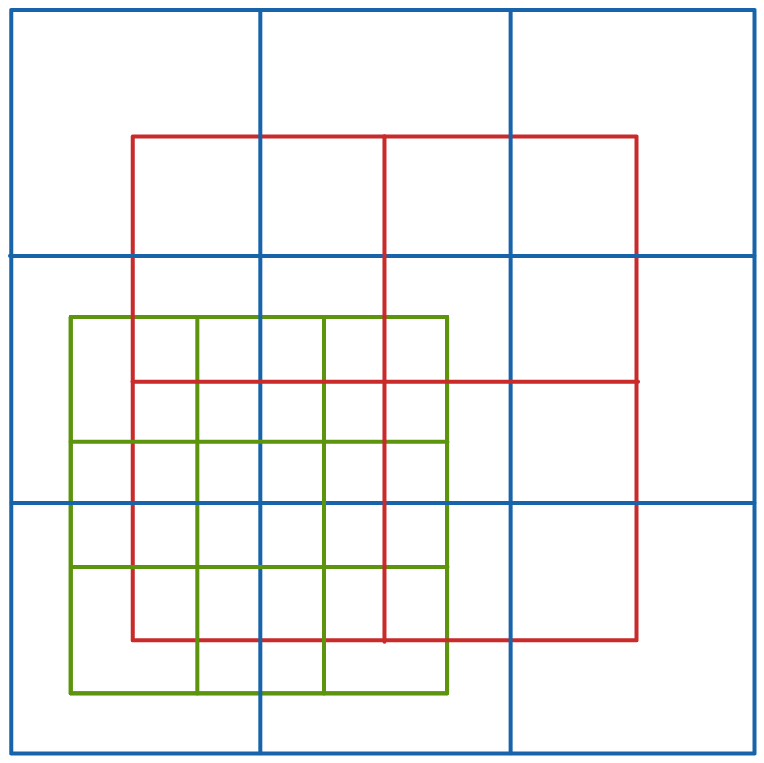
\includegraphics[width=\textwidth]{fourth-child-brick.png}
        \end{subfigure}
    \end{center}
    \caption{Bricks asociados a cada hijo del nodo}
    \label{fig:all_child_bricks}
\end{figure}

Los valores de los vóxeles del brick padre se calculan en 4 etapas distintas, dependiendo de dónde se ubican en el \textit{brick}: Esquinas, bordes, caras, centro.
Cada una de las etapas calcula un valor parcial para un tipo de vóxel.
Es parcial porque para los vóxeles limítrofes con otro nodo, este valor tiene que luego ser agregado con el de los vecinos, con un tipo de \textit{border\_transfer}.

% El cálculo para cada etapa es el mismo para todos los vóxeles dentro de su grupo, por lo que se mostrará únicamente el calculo para un vóxel de cada grupo: esquinas, bordes, caras, y centro.
% En el caso 2D, no existe el vóxel centro.

\begin{figure}
    \centering
    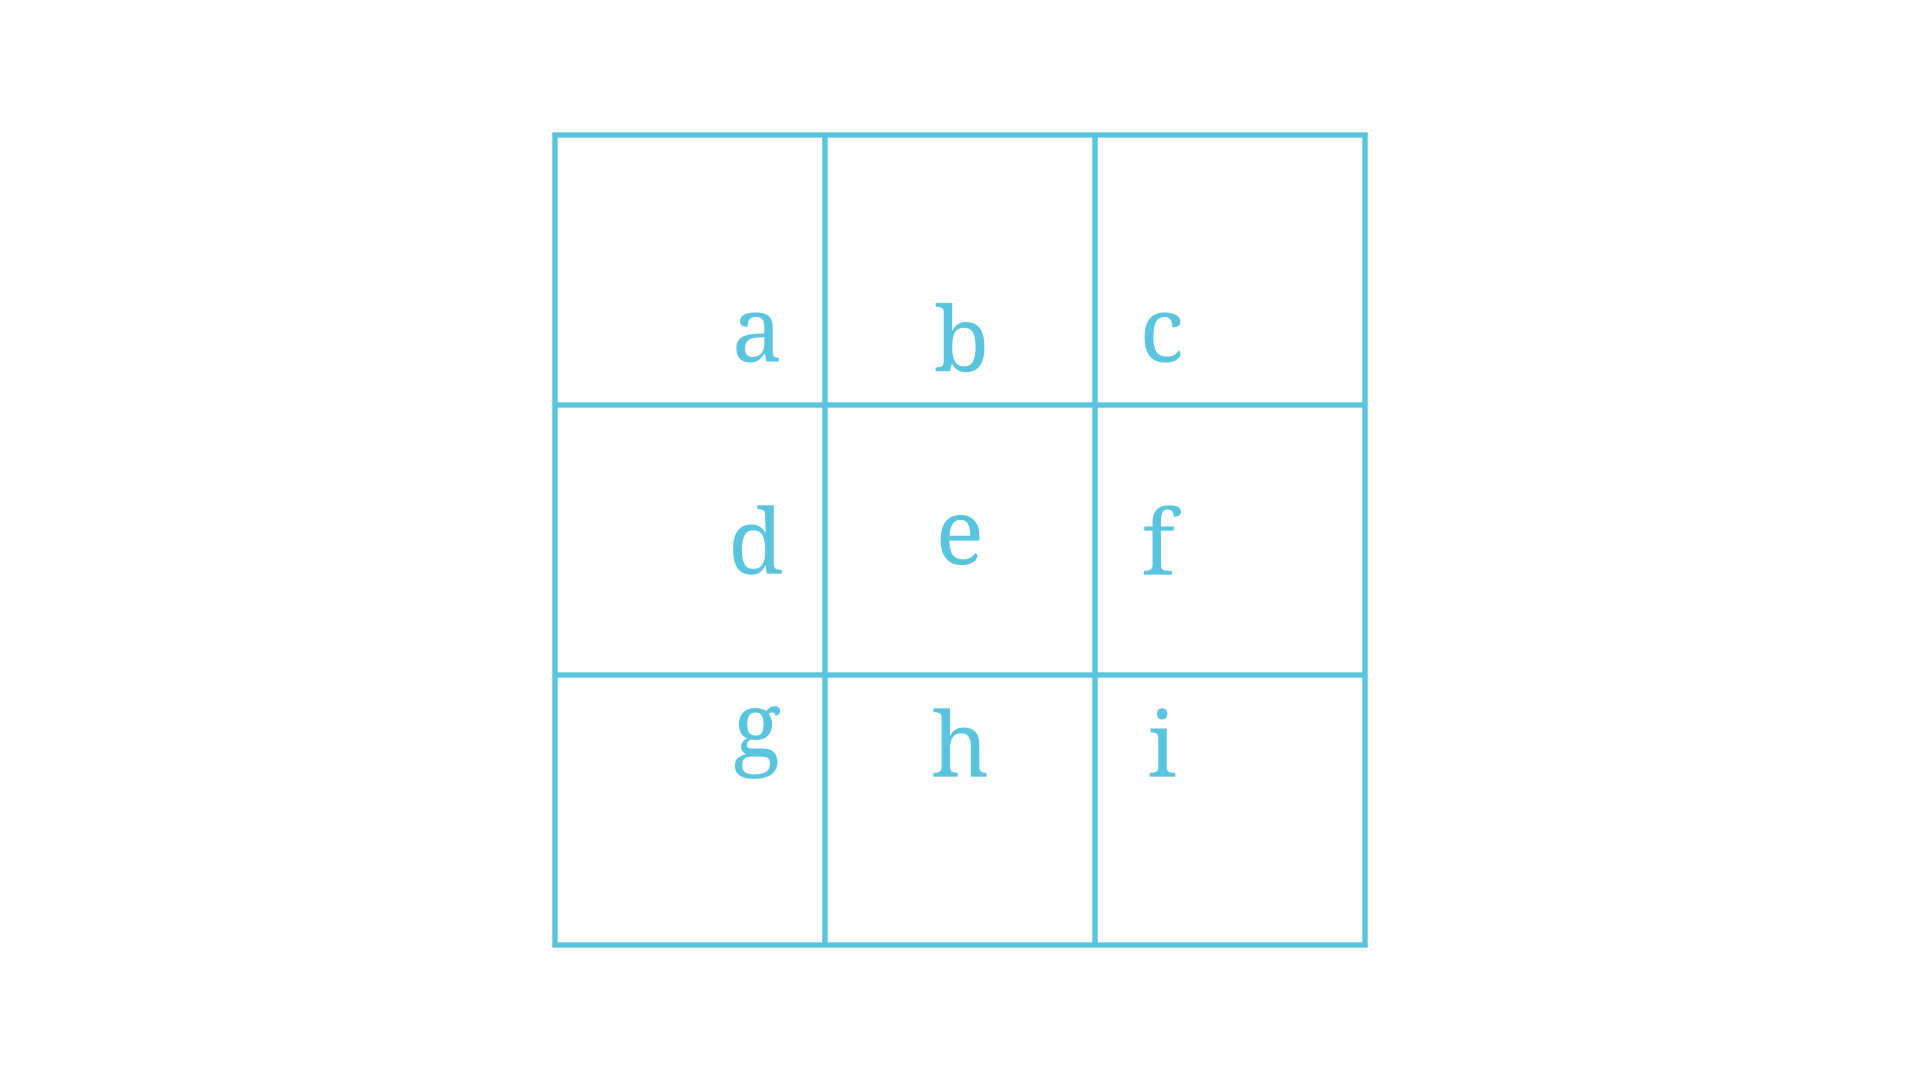
\includegraphics[width=.5\textwidth]{brick-voxel-naming.png}
    \caption{Una posible forma de referirse a cada vóxel de un brick}
    \label{fig:brick-voxel-naming}
\end{figure}

Dado el vóxel superior izquierdo de la figura \ref{fig:svo_filtering_corners}, se considera solo el brick del hijo superior izquierdo del nodo.
De ese brick, se consideran los vóxeles amarillos en la figura.
El valor final del vóxel del padre se calcula promediando los valores de los vóxeles del hijo, pesados por el porcentaje de solapamiento.
Si nombramos los vóxeles del brick hijo $a, \cdots, i$ y los del brick padre $a', \cdots, i'$, como en la figura \ref{fig:brick-voxel-naming}, entonces el valor del vóxel del padre se calcula como:

$$
a' = a + b * \frac{1}{2} + d * \frac{1}{2} + e * \frac{1}{4}
$$

En el caso tridimensional, hay que agregar un quinto factor multiplicado por $\frac{1}{8}$.

% Esto resulta en un kernel gaussiano. % TODO: Alguna referencia sobre kernels gaussianos? Si no no lo mencionamos

\begin{figure}
    \centering
    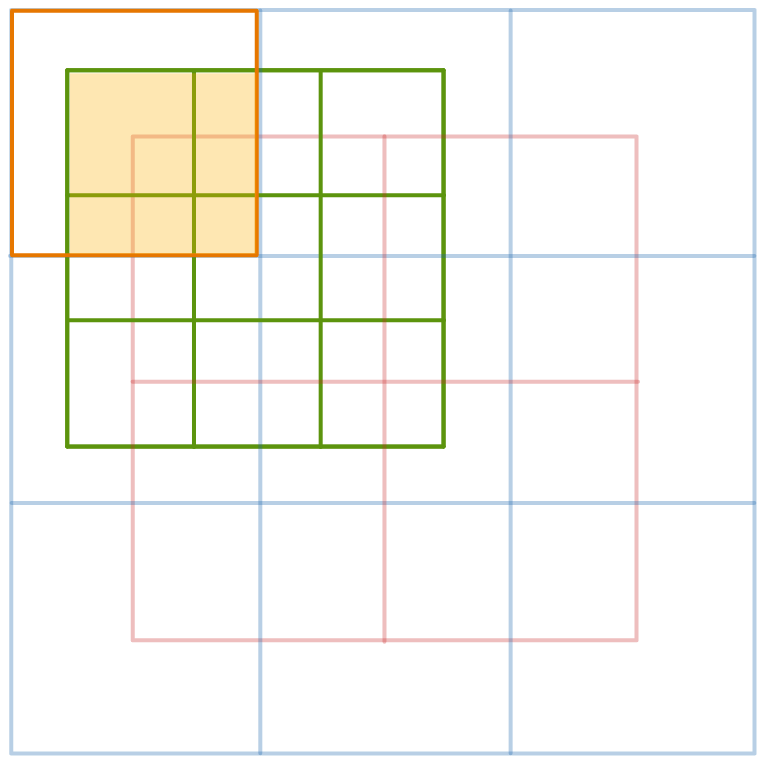
\includegraphics[width=.25\textwidth]{svo-filtering-corner.png}
    \caption{
        Filtrado para un vóxel esquina.
        Se puede ver el vóxel del brick padre cuyo valor se quiere calcular, junto con el brick del hijo y su solapamiento con este vóxel.
    }
    \label{fig:svo_filtering_corners}
\end{figure}

De la misma manera se calculan los vóxeles de los bordes y de las caras, solo que en esos casos se usan más de un brick hijo, como se puede ver en las figuras \ref{fig:svo_filtering_edges} y \ref{fig:svo_filtering_faces}.

\begin{figure}
    \begin{center}
        \begin{subfigure}{.24\textwidth}
            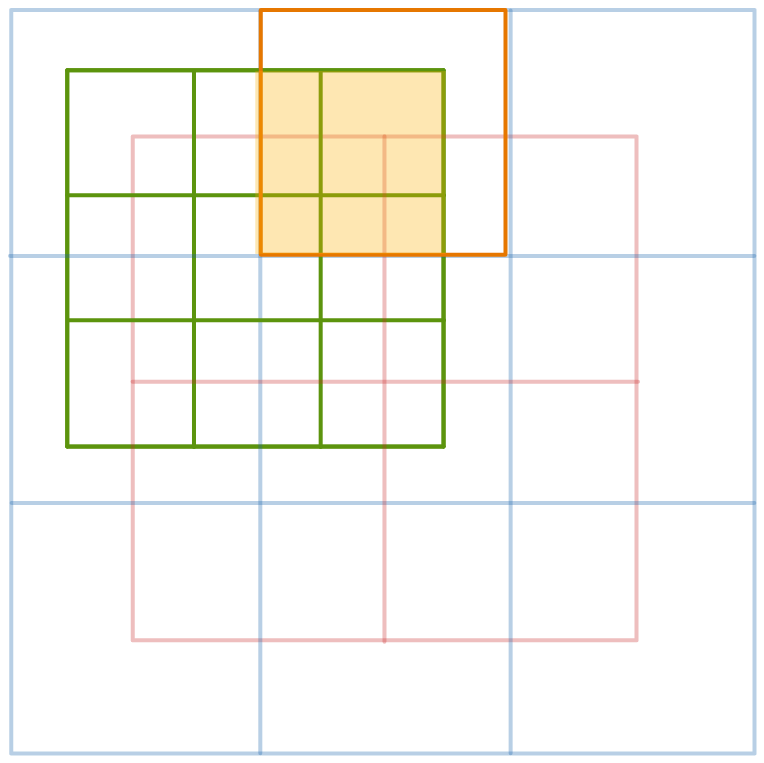
\includegraphics[width=\textwidth]{svo-filtering-edge-1.png}
        \end{subfigure}
        \begin{subfigure}{.24\textwidth}
            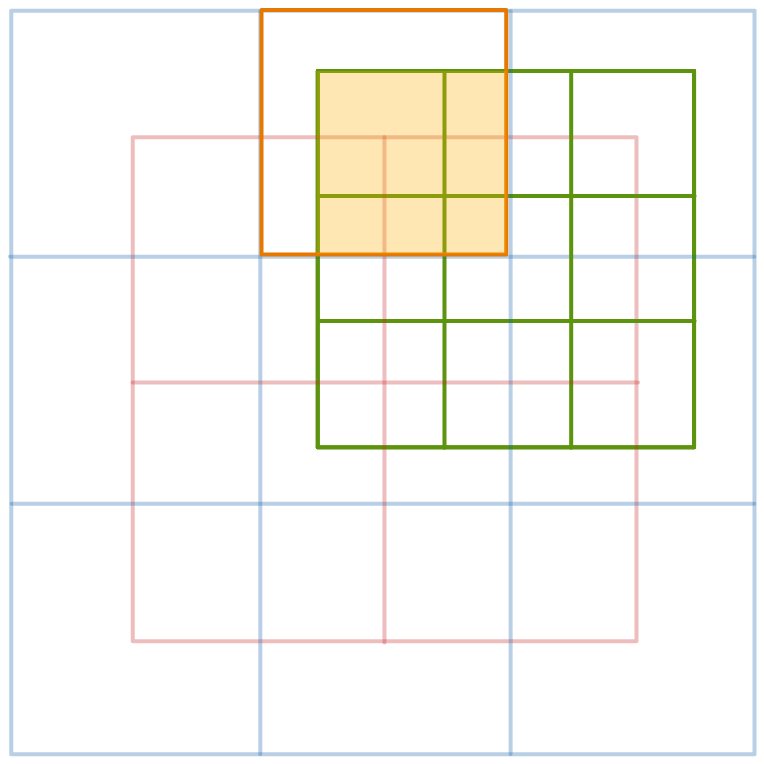
\includegraphics[width=\textwidth]{svo-filtering-edge-2.png}
        \end{subfigure}
    \end{center}
    \caption{Filtrado para un vóxel borde}
    \label{fig:svo_filtering_edges}
\end{figure}

\begin{figure}
    \begin{center}
        \begin{subfigure}{.24\textwidth}
            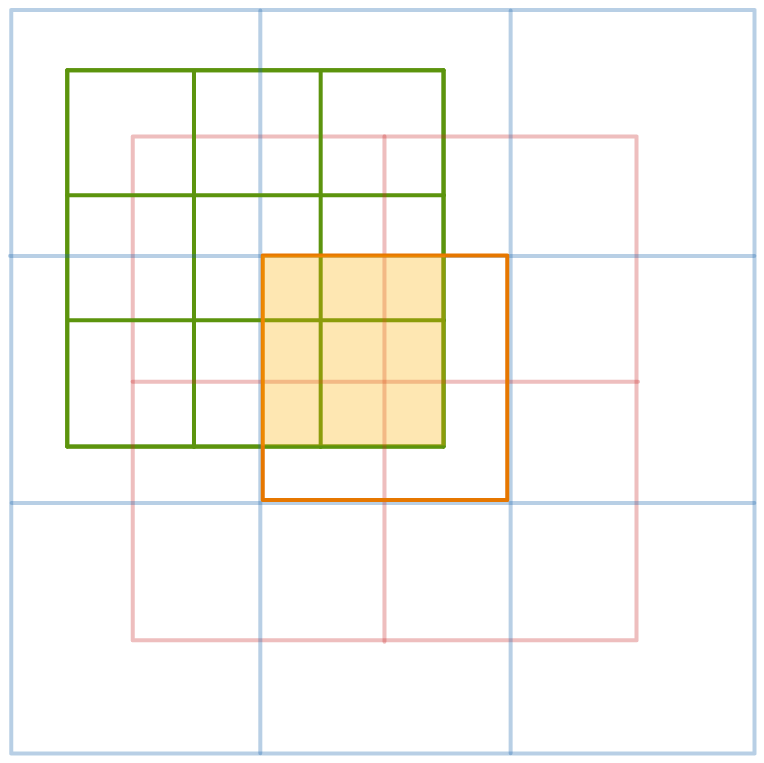
\includegraphics[width=\textwidth]{svo-filtering-face-1.png}
        \end{subfigure}
        \begin{subfigure}{.24\textwidth}
            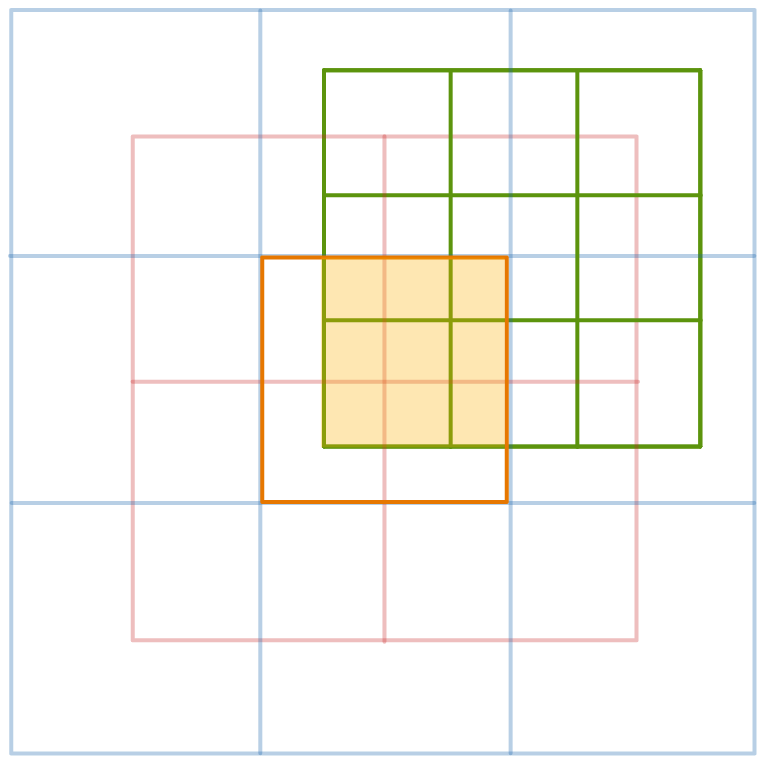
\includegraphics[width=\textwidth]{svo-filtering-face-2.png}
        \end{subfigure}
        \begin{subfigure}{.24\textwidth}
            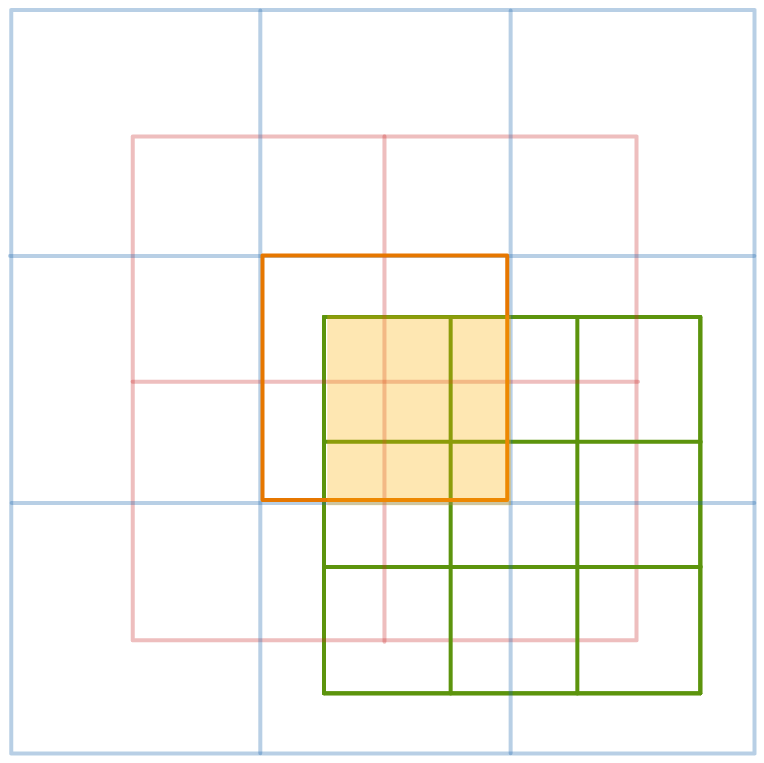
\includegraphics[width=\textwidth]{svo-filtering-face-3.png}
        \end{subfigure}
        \begin{subfigure}{.24\textwidth}
            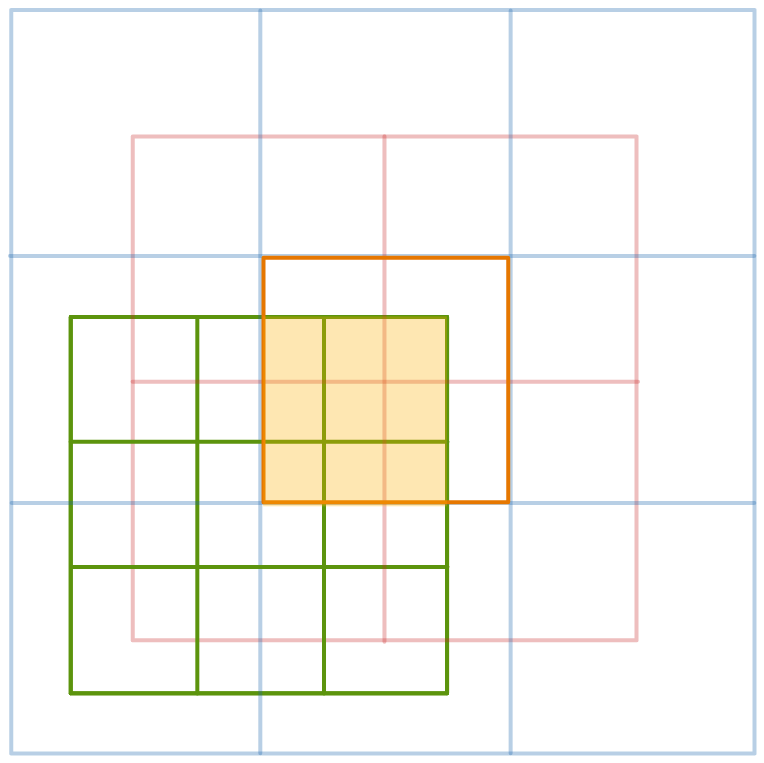
\includegraphics[width=\textwidth]{svo-filtering-face-4.png}
        \end{subfigure}
    \end{center}
    \caption{Filtrado para un vóxel cara}
    \label{fig:svo_filtering_faces}
\end{figure}

% TODO: Solo traer de vuelta si realmente usamos normales en el código.
% Si los vóxeles almacenan normales, estas se promedian como se mencionó en la sección \ref{sec:normal_filtering}.

\subsection{Filtrado anisotrópico}

El filtrado descrito en la sección anterior resulta en vóxeles con valores independientes del punto de vista.
Una característica deseable es que los valores de oclusión y opacidad dependan del punto de vista del observador, lo cual se logra en este caso guardando mas de un valor por vóxel para estas propiedades.
Es muy útil a la hora de representar un atributo en una escena 3D.

Para ilustrar el punto anterior, consideremos una escena compuesta únicamente por una pared fina.
Dado un vóxel de un nodo en un nivel alto del árbol, el nodo representa una gran región del espacio.
La región contiene únicamente una pared que pasa por su centro, y el resto de la escena es espacio vacío.
Con el filtrado presentado en las secciones anteriores, llamado \textbf{isotrópico}, el vóxel tendrá un unico valor de opacidad que, al representar un espacio mayormente vacío, tendra un valor bajo.
Sin embargo, se observa que la percepción de la pared es muy distinta si se la ve de frente o de costado.
Como se muestra en la figura \ref{fig:anisotropic-thin-wall}, la pared vista de frente es opaca, pero vista de costado su superficie visible es practicamente nula, lo cual se asemeja a una superficie transparente.

La solución propuesta por Crassin \cite{voxel-cone-tracing} consiste en realizar el filtrado 6 veces por vóxel, uno por cada dirección alineada con los ejes: X, -X, Y, -Y, Z, -Z; y tener en cuenta la dirección a la hora de promediar los valores.
Cada uno de los 6 valores representa el voxel visto desde una de las 6 direcciones previamente mencionadas. Por lo tanto si se observa el vóxel desde una direccion arbitraria, se calcula su oclusión y color a través de la interpolación de las tres direcciones mas cercanas.
Este tipo de filtrado se denomina \textbf{anisotrópico}, dado que depende de la dirección con que se observe al vóxel.

\begin{figure}
    \centering
    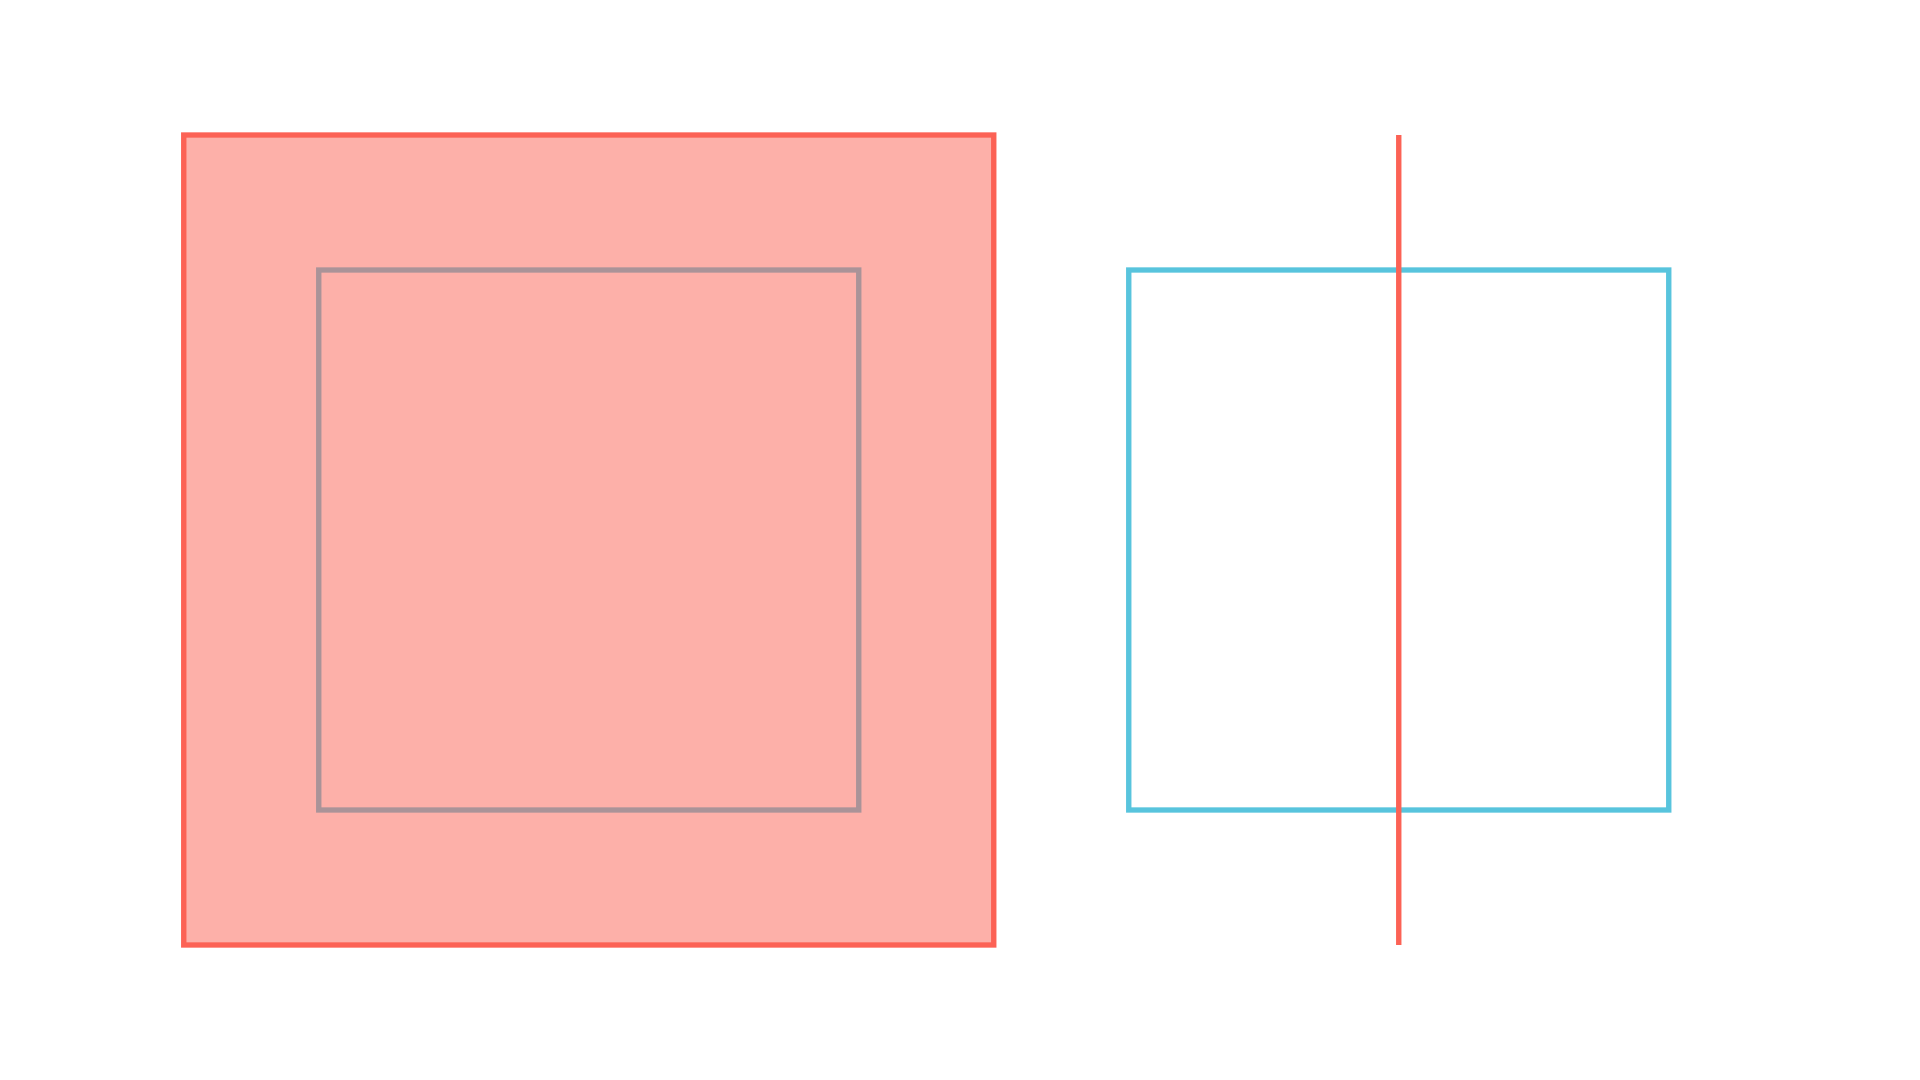
\includegraphics[width=.5\textwidth]{anisotropic-thin-wall.png}
    \caption{
        Vóxel que contiene una pared fina.
        En la izquierda, la pared se ve de frente.
        En la derecha, se ve de costado.
        Se espera que el valor del vóxel refleje esta diferencia entre las direcciones de vista.
    }
    \label{fig:anisotropic-thin-wall}
\end{figure}

Dada una dirección, por ejemplo, de izquierda a derecha, se parte de los vóxeles de la izquierda y se calcula un valor para cada fila, partiendo de estos y yendo hacia los vóxeles de la derecha.
Llamémosle al valor de cada fila \textbf{valor direccional}.
En la figura \ref{fig:svo_filtering_anisotropic} se pueden ver todos los valores direccionales que deben ser calculados para un brick en 2D, para todas las direcciones.
Para cada fila, se ejecuta un algoritmo de acumulación de opacidad que va avanzando en la dirección dada.
Si el algoritmo llega a opacidad 1, termina y devuelve el valor direccional para esa fila.

\begin{figure}
    \begin{center}
        \begin{subfigure}{.24\textwidth}
            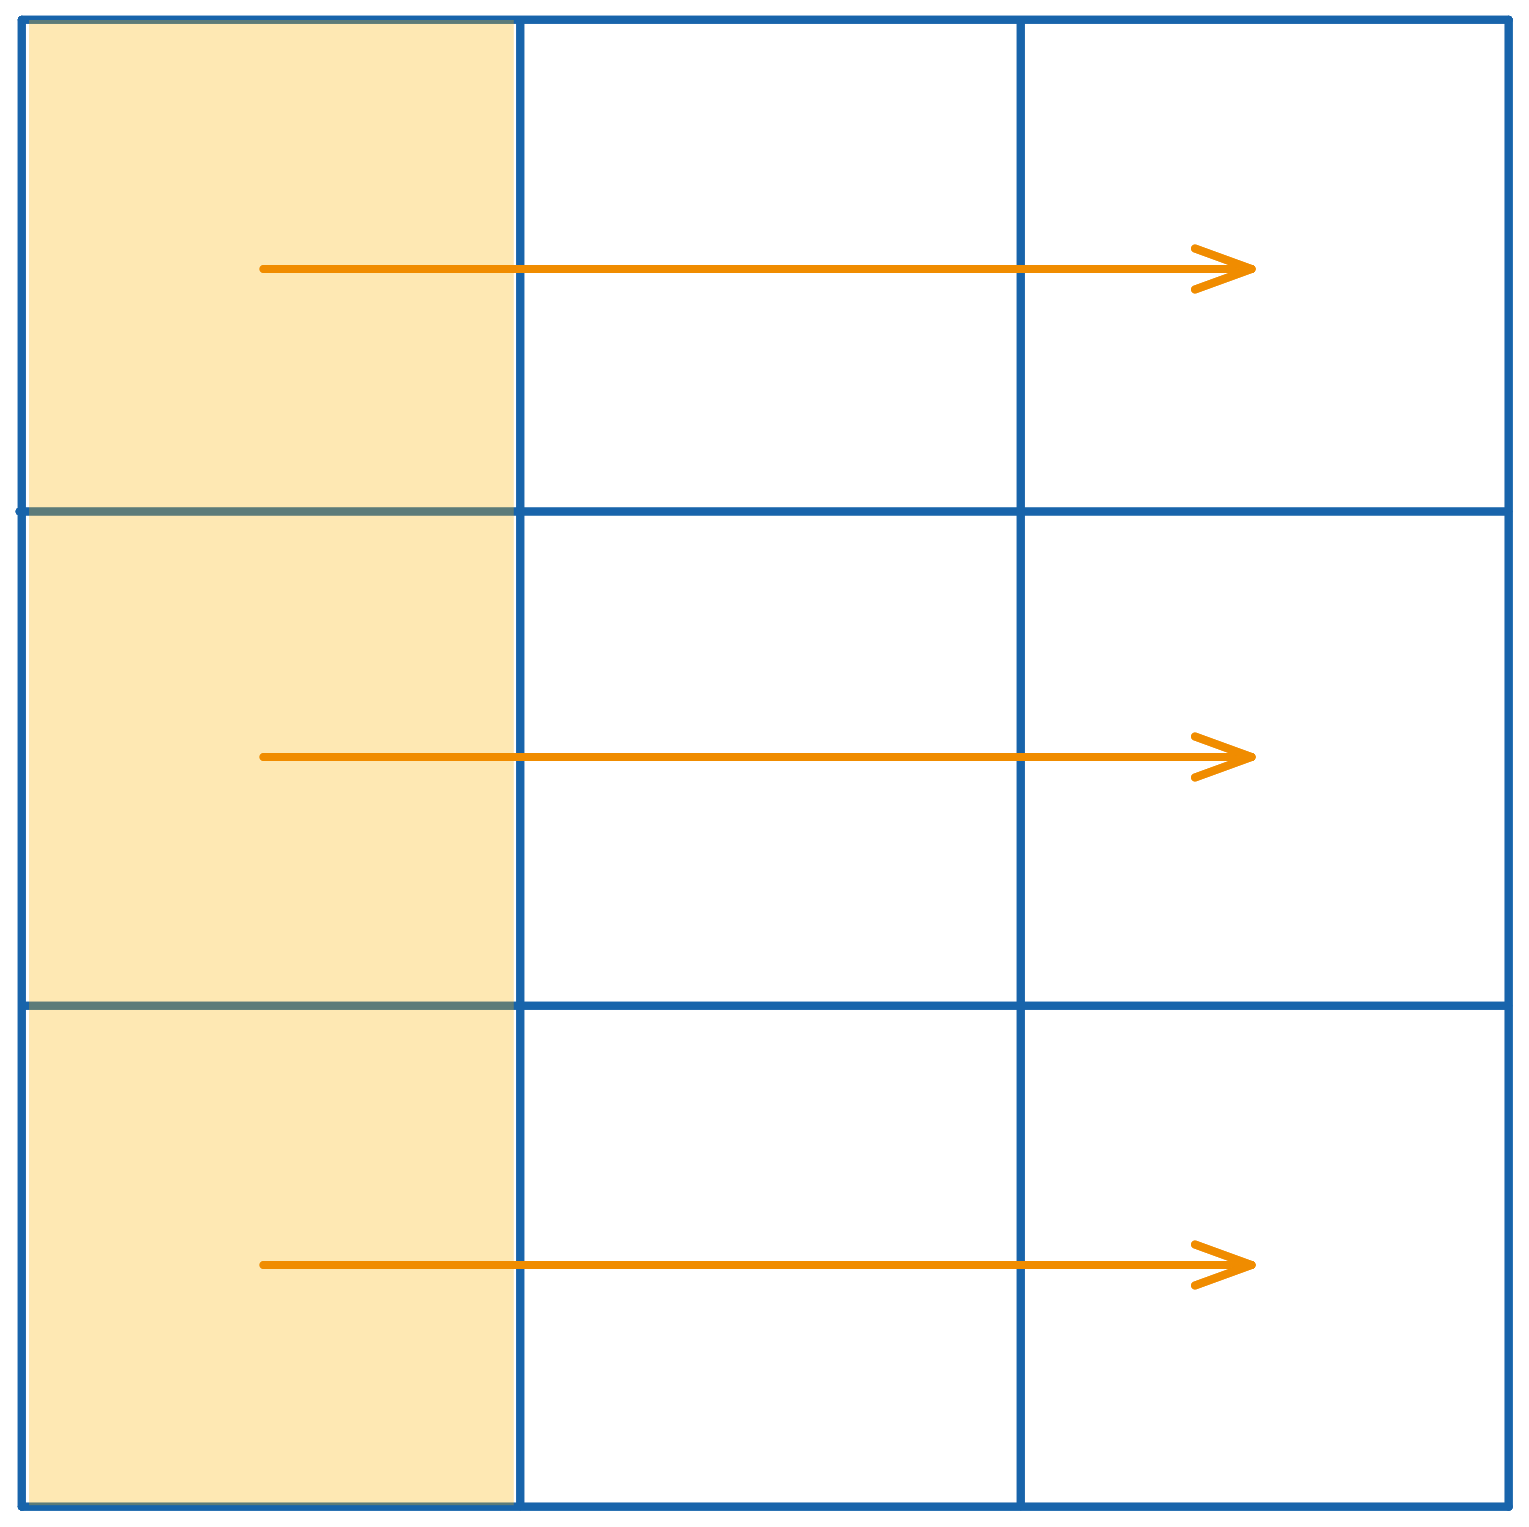
\includegraphics[width=\textwidth]{anisotropic-filtering-x.png}
        \end{subfigure}
        \begin{subfigure}{.24\textwidth}
            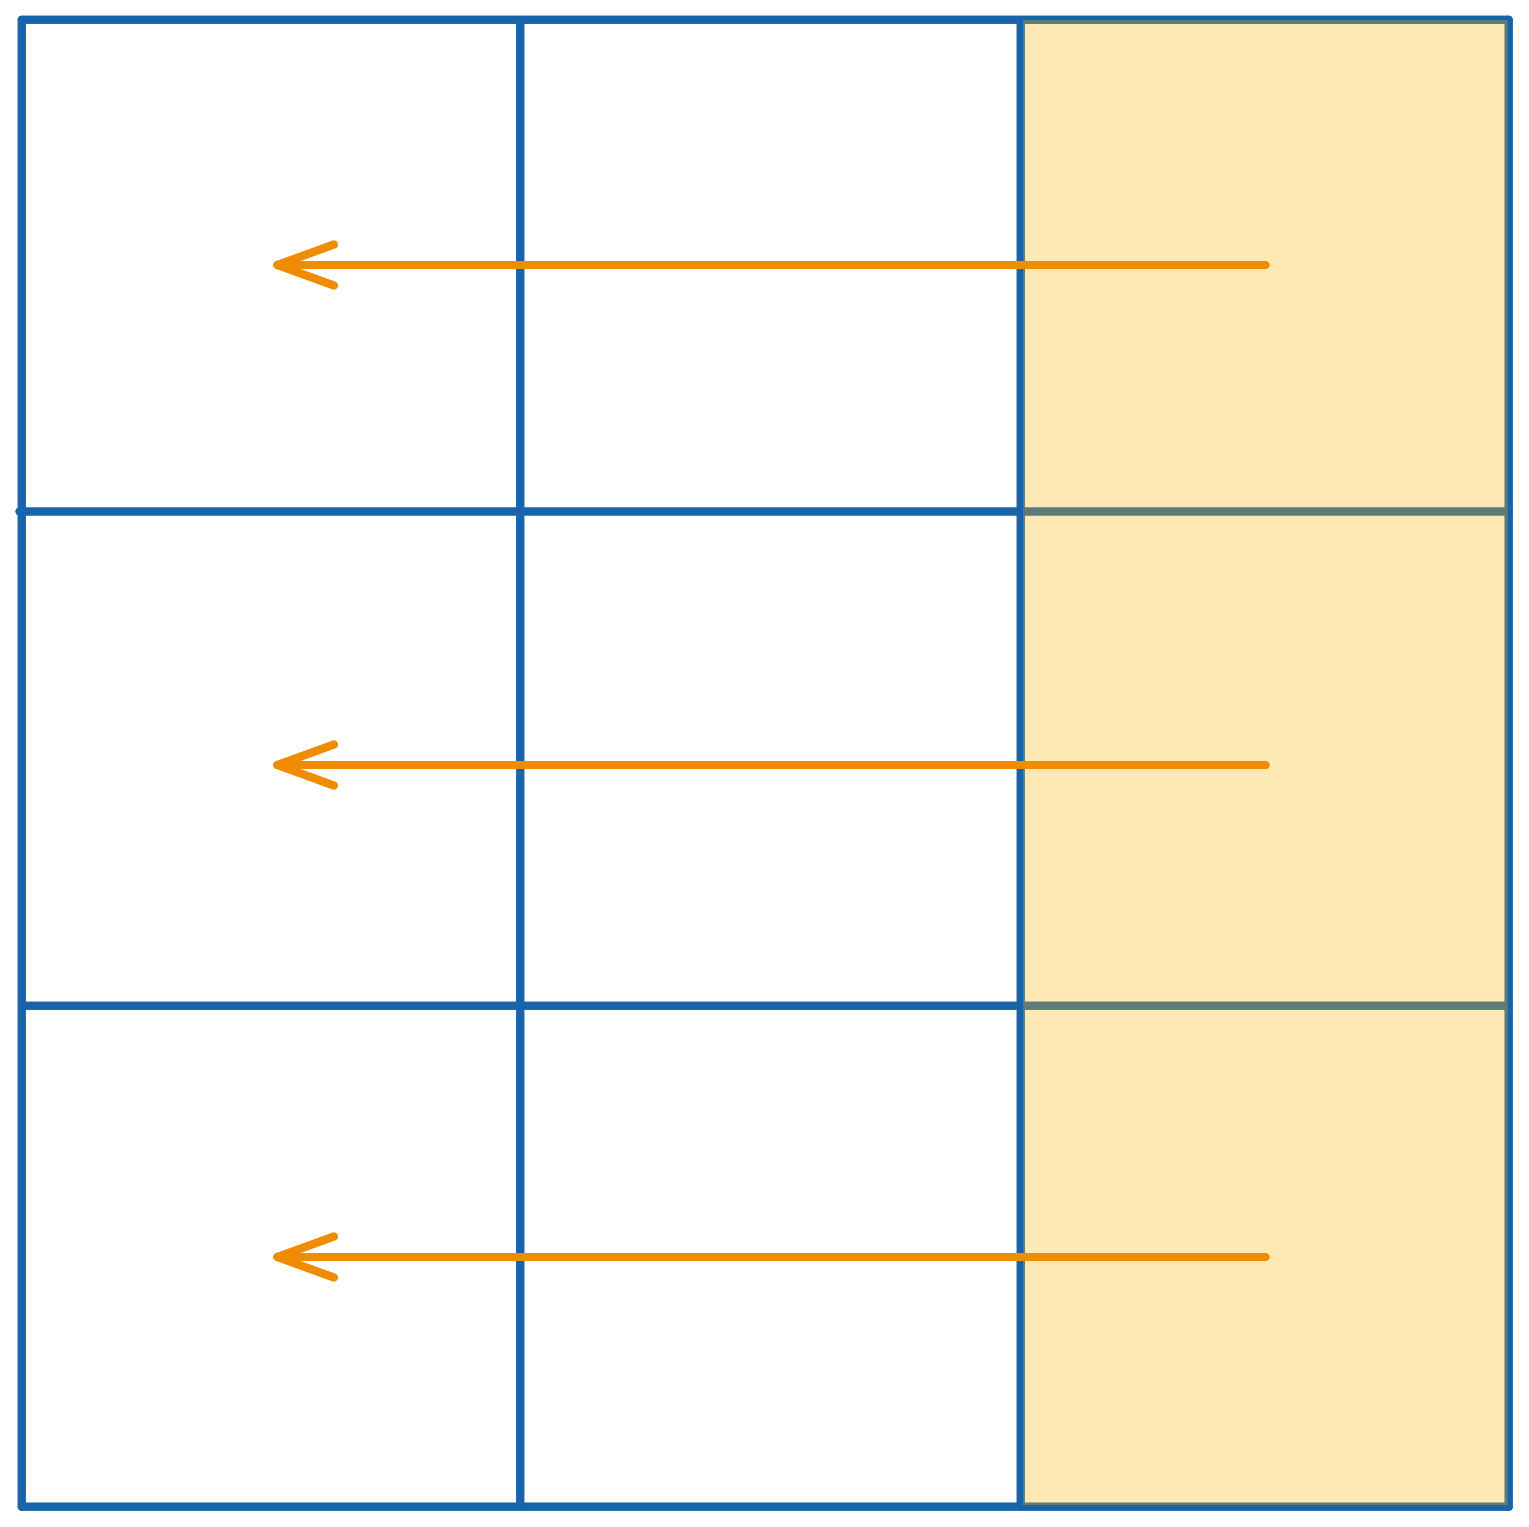
\includegraphics[width=\textwidth]{anisotropic-filtering-x-neg.png}
        \end{subfigure}
        \begin{subfigure}{.24\textwidth}
            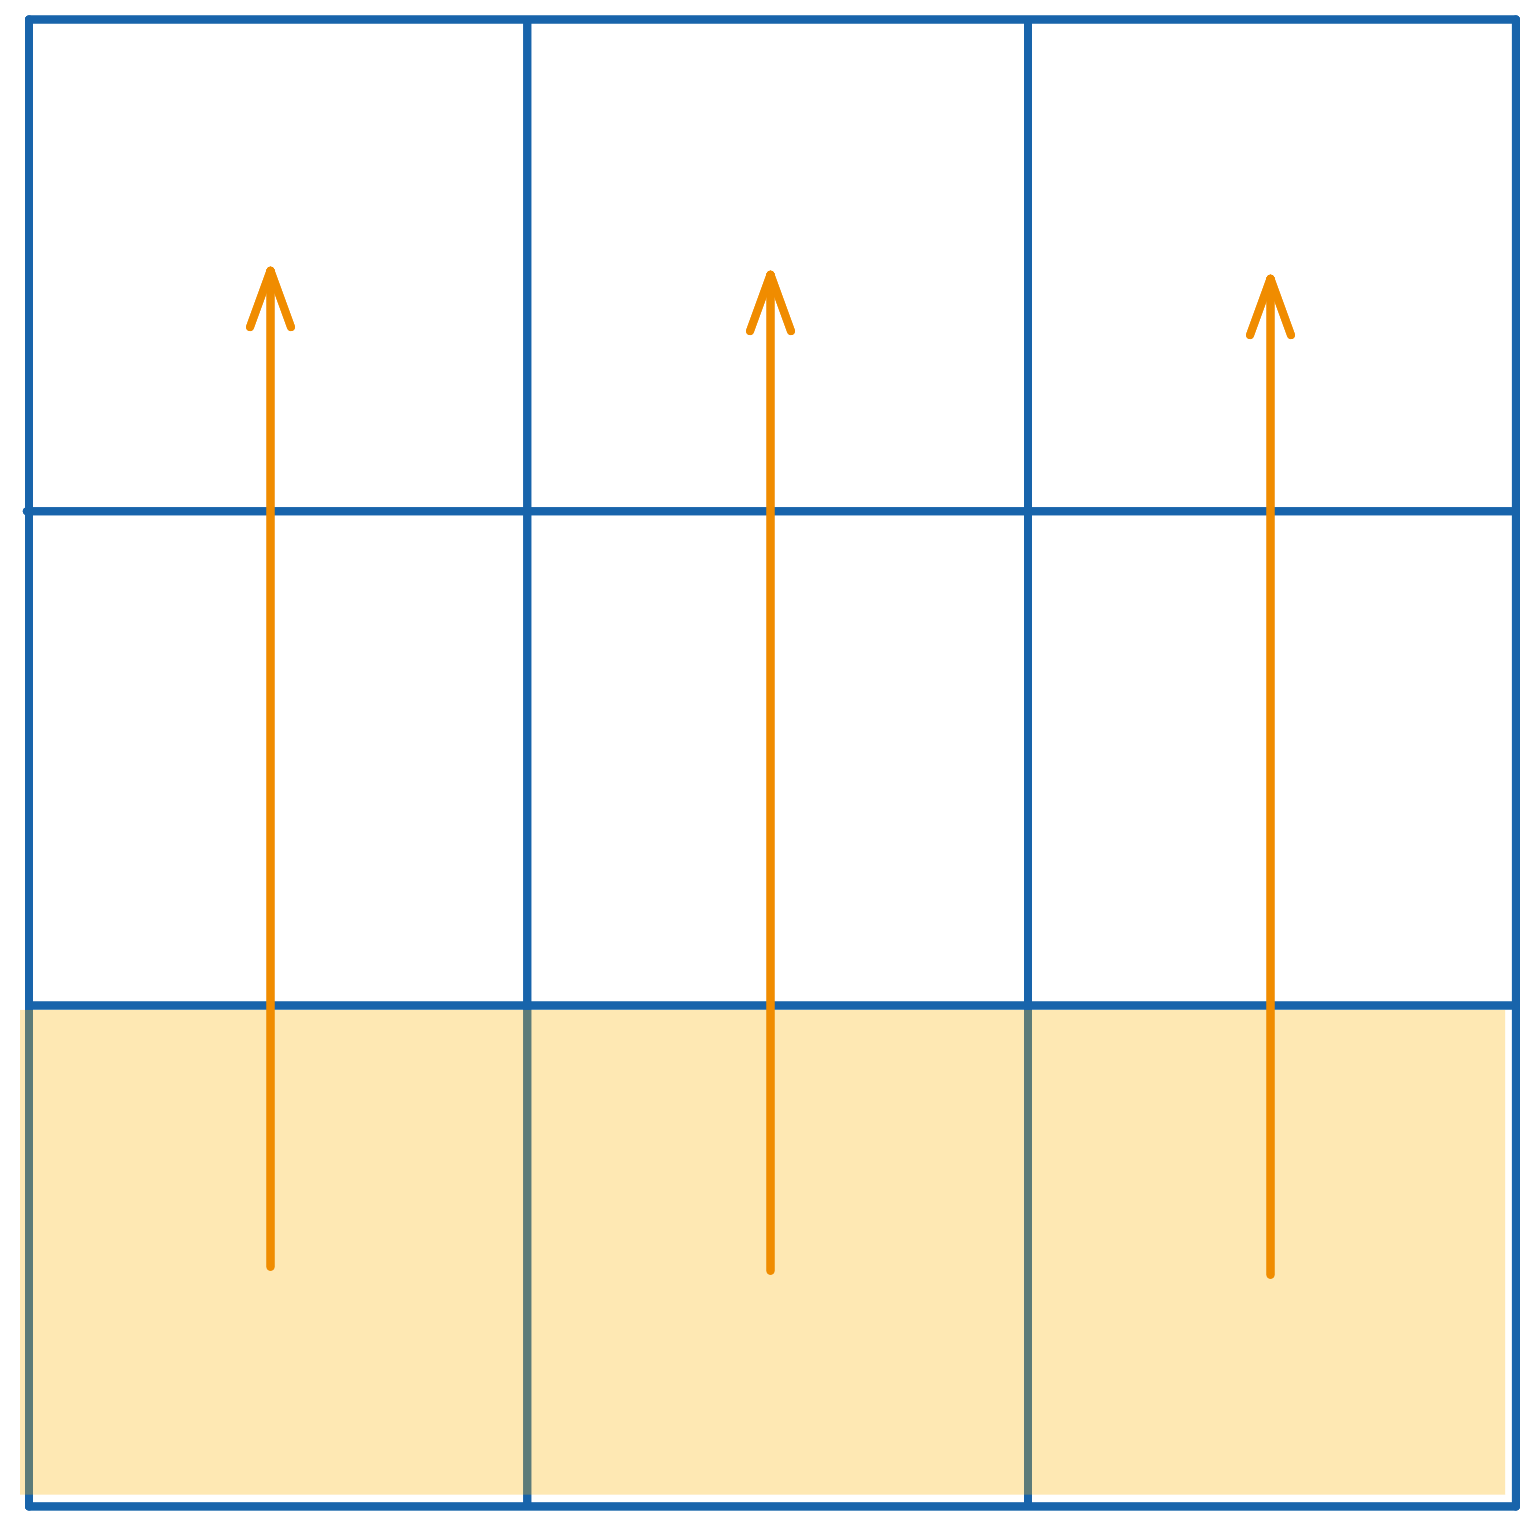
\includegraphics[width=\textwidth]{anisotropic-filtering-y.png}
        \end{subfigure}
        \begin{subfigure}{.24\textwidth}
            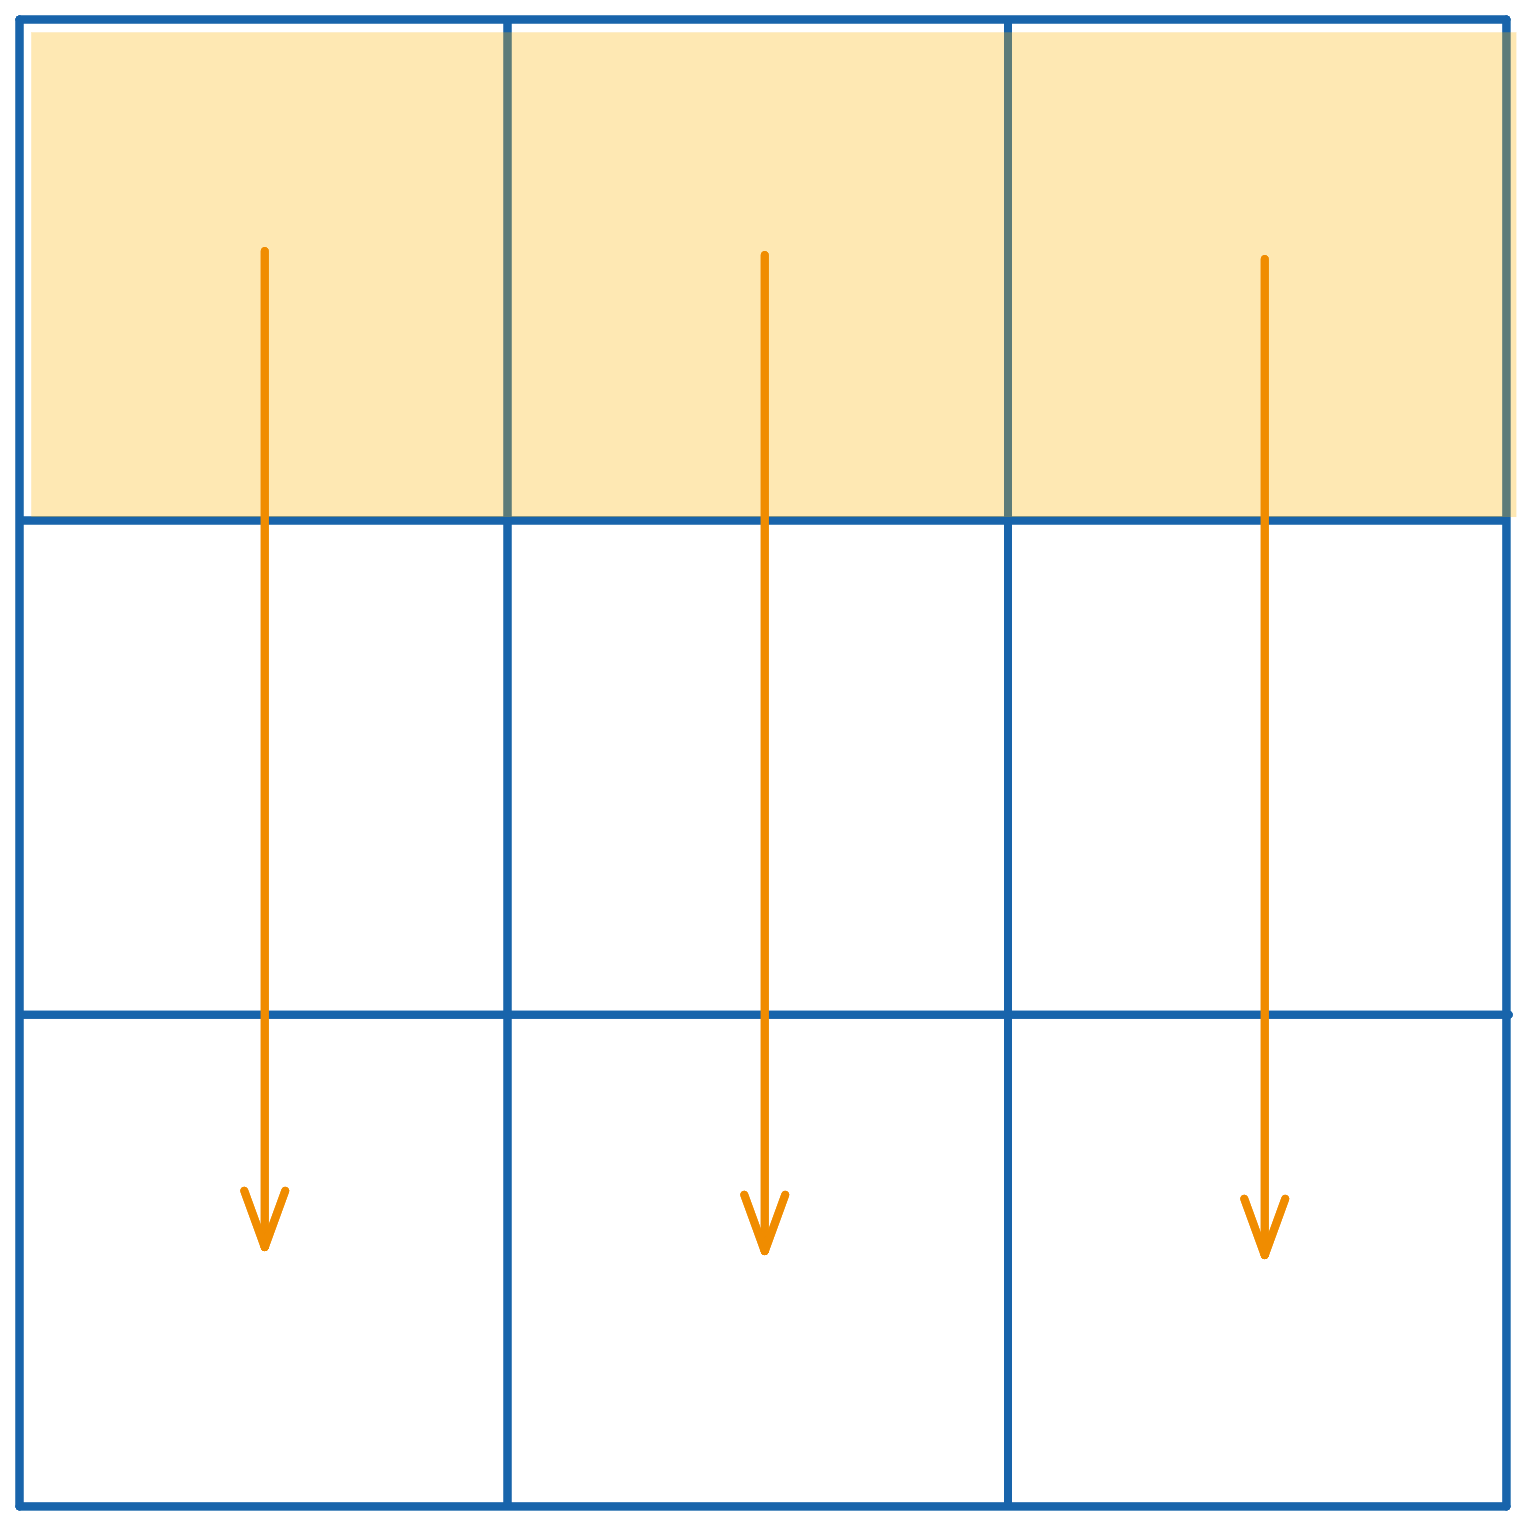
\includegraphics[width=\textwidth]{anisotropic-filtering-y-neg.png}
        \end{subfigure}
    \end{center}
    \caption{Filtrado anisotrópico en todas las direcciones}
    \label{fig:svo_filtering_anisotropic}
\end{figure}

El filtrado anisotrópico soluciona situaciones como la de la pared mencionada anteriormente.
Para el caso de la pared fina, el vóxel que contiene la pared es opaco en la dirección paralela a la normal de la pared y prácticamente transparente en cualquiera de las perpendiculares.

\section{Inyección de fotones}\label{sec:photon-injection}

Hasta ahora tenemos la estructura de datos creada, conteniendo el color y opacidad de toda la escena en las hojas y un promedio de los niveles inferiores en todos los nodos interiores.
El objetivo del algoritmo es la iluminación global de una escena, por lo que necesitamos información de la luz.
En este paso, lanzamos fotones a partir de la fuente de luz de la escena, similar a como se hace en \textit{photon mapping}, lo cual se logra utilizando el ducto de rasterización.

Se rasteriza la escena desde el punto de vista de la luz para generar una textura 2D.
En lugar de tener colores en cada téxel de la textura, se almacenan las posiciones de los objetos de la escena.
La existencia de una posición en un texel de la textura significa que esa posición es visible desde la luz, por lo cual debe recibir un fotón.
Las posiciones son utilizadas para recorrer el octree y almacenar los fotones en vóxeles de sus hojas.

Los fotones que se almacenan en los vóxeles del árbol, la \textbf{irradiancia}, es el flujo lumínico recibido por cada superficie.
Luego pasan por el mismo proceso de \textit{border\_transfer} y filtrado que el color.
El \textit{border\_transfer} suma en lugar de promediar en este caso, dado que ambos lados de la frontera aportan a la cantidad de fotones total.
El filtrado funciona de la misma manera.

La etapa de construcción debe realizarse solo una vez, mientras que, al soportar luces dinámicas, esta etapa debe ejecutarse cada vez que la luz se mueva.
En esos casos, toda la irradiancia del árbol vuelve a cero y se vuelve a correr el programa que lanza los fotones, y lo llamaremos la actualización de la estructura.

% TODO: Quedó extremadamente corta esta parte
% Estaría bueno hablar de las optimizaciones? Te hacen perder un poco

\section{\textit{Cone tracing}}\label{sec:cone_tracing}

Como se comentó brevemente al inicio del capítulo, el trazado de conos se realiza en el \textit{fragment shader} del ducto de rasterización.
La entrada al algoritmo de \textit{cone tracing} son los \textit{geometry buffers} que contienen los valores de la escena, ya habiendo descartado los vértices fuera de vista.
El algoritmo de trazado de conos es ejecutado para cada píxel de los geometry buffers para calcular el color final.

Dado un punto de origen, se lanza uno o varios conos con cierta dirección y apertura, dependiendo del efecto que se quiere lograr.
% TODO: Tema de las normales todo considerando el hemisferio hacia el lado de la normal del punto.

Para cada cono, se parte desde su origen y se avanza en la dirección de su eje tomando pasos de cierto tamaño.
Esto se conoce como \textit{ray marching}. % TODO: No se si está bueno poner el nombre sin haberlo mencionado antes
Después de cada paso tomado, se calcula el diámetro del cono en ese punto $P$.
Luego se encuentra el nivel del octree con el menor tamaño posible de voxel que cumpla la condición de ser mayor que el diámetro del cono.
Dado ese nivel y la posición del punto $P$, se recorre el octree y se encuentra el nodo que correspondiente a ese nivel que incluye el punto.
Ese nodo tiene un brick asociado, cuyos vóxeles tienen los valores prefiltrados, conseguidos en \ref{design:filtering}.
Se usa el valor del vóxel que corresponde con la posición y se acumula. En caso de vóxeles anisotrópicos, también depende de la direccion del eje del cono.
Se sigue avanzando paso a paso acumulando valores hasta satisfacer un criterio de parada.
El algoritmo de \textit{cone tracing} en si es simple dados todos los pasos anteriores.

Cada cono calcula un color $c$ y una opacidad $\alpha$.
Si en cada paso consideramos $c$ y $\alpha$ como los valores hasta el momento, y $c_2$ y $\alpha_2$ como los valores nuevos encontrados en el vóxel del paso, entonces en cada paso los valores de $c$ y $\alpha$ se calculan de la siguiente manera:

$$
\begin{cases}
    c = \alpha c + (1 - \alpha) \alpha_2 c_2 \\
    \alpha = \alpha + (1 - \alpha) \alpha_2
\end{cases}
$$

Para la luz indirecta difusa, se lanzan conos para cubrir el hemisferio centrado en la normal del punto.
En la mayoría de los casos, 5 conos anchos difusos dan un buen resultado.
Cada cono acumula el color de los vóxeles con los que se encuentra multiplicado por la cantidad de fotones.
Esto logra un efecto de \textit{light bleed}, donde las superficies adquieren color de otras superficies cercanas que reciben y dispersan luz.

Para la luz indirecta especular, se lanza un solo cono fino en la dirección de reflexión.
El cono, al ser más fino, es rápidamente ocluido por nodos de niveles más bajos, con lo que el reflejo tiene mejor definición.
Si se utiliza un mayor ángulo de apertura del cono, el reflejo se ve más turbio, simulando una superficie menos pulida.

\section{Oclusión ambiental}

La oclusión ambiental es una técnica de rendering que se usa para calcular qué tan expuesto está cada punto de una escena a la luz ambiental.
\textit{Cone tracing} se puede usar para calcular este valor.
El efecto no aporta más al realismo de una escena una vez que se usan técnicas de iluminación indirecta, pero es un buen paso previo para ver el funcionamiento del algoritmo.

Para calcularlo, se lanzan varios conos, cubriendo el hemisferio centrado en la normal de la superficie en el punto.
El único valor necesario es la opacidad.
A medida que se viaja a lo largo de un cono, se va acumulando la opacidad de los vóxeles correspondientes.
Se define una distancia máxima y el criterio de parada es cuando el punto a lo largo del cono pasa esa distancia máxima, o la oclusión llega a 1.

\section{Conos de sombra}

De la misma manera que el trazado de rayos logra sombras lanzando un rayo hacia la fuente de luz, mientras que en cone tracing se logran lanzando un cono hacia la fuente de luz.
El cono toma en cuenta únicamente la opacidad y su criterio de parada es alcanzar la luz o 1 de opacidad antes.
El beneficio de que sea un cono en lugar de un rayo, y de tener la estructura jerárquica del \textit{octree}, es que se logran sombras suaves, sin necesidad de tener que tomar muchas muestras y promediarlas.

% END.
